\documentclass[conference,a4paper]{IEEEtran}
\IEEEoverridecommandlockouts

% Some very useful LaTeX packages include:
% (uncomment the ones you want to load)
\usepackage[utf8]{inputenc}


% *** CITATION PACKAGES ***
%
\usepackage{cite}


% *** GRAPHICS RELATED PACKAGES ***
%
\usepackage[pdftex]{graphicx}
% declare the path(s) where your graphic files are
\graphicspath{{./Images/}}
% and their extensions so you won't have to specify these with
% every instance of \includegraphics
% \DeclareGraphicsExtensions{.PDF,.jpeg,.png}
\makeatletter
\newcommand\footnoteref[1]{\protected@xdef\@thefnmark{\ref{#1}}\@footnotemark}
\makeatother
% https://tex.stackexchange.com/a/35044

% *** MATH PACKAGES ***
%
\usepackage[cmex10]{amsmath}
\usepackage[detect-all]{siunitx}

% *** SPECIALIZED LIST PACKAGES ***
%
\usepackage{algorithmic}


% *** ALIGNMENT PACKAGES ***
%
%\usepackage{array}

%\usepackage{mdwmath}
%\usepackage{mdwtab}

% IEEEtran contains the IEEEeqnarray family of commands that can be used to
% generate multiline equations as well as matrices, tables, etc., of high
% quality.

%\usepackage{eqparbox}

% *** SUBFIGURE PACKAGES ***
%\usepackage[tight,footnotesize]{subfigure}

%\usepackage[caption=false]{caption}
%\usepackage[font=footnotesize]{subfig}

\usepackage[caption=false,font=footnotesize]{subfig}
\usepackage{tablefootnote}
\usepackage{capt-of}
\usepackage{needspace}
\usepackage[flushleft]{threeparttable}

% *** MATH PACKAGES ***
\usepackage{amsmath}

\DeclareMathOperator{\arctantwo}{arctan2}
\DeclareMathOperator{\sinsq}{sin^2}

% *** FLOAT PACKAGES ***
%
%\usepackage{fixltx2e}

%\usepackage{stfloats}

%\fnbelowfloat

% *** PDF, URL AND HYPERLINK PACKAGES ***
%
\usepackage[obeyspaces]{url}
\usepackage{xurl}

% Advanced table environment
\usepackage{booktabs}

% correct bad hyphenation here
\hyphenation{op-tical net-works semi-conduc-tor}

% Create separator commands:
\let\oldsection\section
\renewcommand{\section}[1]{
  \setlength{\parskip}{0em}
  \setlength{\parindent}{0pt}
  \oldsection{#1}
}

\let\oldsubsection\subsection
\renewcommand{\subsection}[1]{
  \setlength{\parskip}{0.5em}
  \setlength{\parindent}{0pt}
  \oldsubsection{#1}
}

\newcommand{\ParagraphSeperator}{
  \setlength{\parskip}{0em}
  \setlength{\parindent}{10pt}
}


\begin{document}

% paper title
% can use linebreaks \\ within to get better formatting as desired
\title{TruggySense: Hardware and Firmware Redesign for Reproducibility}

% author names and affiliations
\author{
	\IEEEauthorblockN{
		Thomas Kramp\IEEEauthorrefmark{1}, 
		Jan Steckel\IEEEauthorrefmark{1} \IEEEauthorrefmark{2}
	}
	\IEEEauthorblockA{
		\IEEEauthorrefmark{1}Faculty of Applied Engineering: Department of \mbox{Electronics-ICT} - University of Antwerp, Antwerp, Belgium, \\
		\IEEEauthorrefmark{2}Flanders Make Strategic Research Centre, Lommel, Belgium
	}
	\thanks{Master's thesis to obtain the diploma 
			Master of Science in Electronics and Information and Communication Technology. Academic year \mbox{2024-2025}.
			This Master's thesis is an examination document that may not have been corrected for any errors in its final version. 
			Reproduction and copying of this publication or parts thereof are prohibited without the prior written consent of 
			both the supervisor(s) and the author(s). For requests or information regarding the publishing and/or use and/or 
			realization of parts of this publication, please contact the university at which the author is registered.
			Prior written consent of the supervisor(s) is also required for the use of the (original) methods, products, 
			circuits and programmes described in this thesis for industrial or commercial use, and for the submission of this 
			publication for participation in scientific prizes or competitions.

			This document has been assessed by supervisor(s) and/or supervisors in accordance with the faculty 
			Master's thesis regulations.}
}

% make the title area
\maketitle

\ParagraphSeperator
\begin{abstract}
%\boldmath
In this paper a redesign of both hardware and firmware regarding the TruggySense, an off-road Data Acquisition System (DAQ) implemented on a 1/8 Remote-Controlled Vehicle (RCV), is presented.
The system is intended to provide practical and consistent data to enable academic learning opportunities surrounding Advanced Driving Assistance Systems (ADAS).
The TruggySense was able to produce insight into itself, as an RCV, by providing real-time telemetry data and performing four experiments that replicate real-world vehicle behavior~\cite{Elsermans2025}.
The redesign reaffirms this while streamlining its assembly and simplifying the process that allows for future modifications.
\end{abstract}

\ParagraphSeperator
\begin{keywords}
Remote-controlled vehicles, Data acquisition systems
\end{keywords}

\section{Introduction}
\ParagraphSeperator
The interest in autonomous vehicles (AV) has been growing over the past decades, for both commercial and military applications~\cite{Algahtani2019}.
However, research towards developing cost-effective AVs is limited~\cite{Brown2022, Baumann2024}, as it usually focuses on urban environments.
Using smaller-scale models is a more cost-effective method~\cite{Li2024}, and enables the testing and validation of the algorithms and techniques that can later be implemented on their full-scaled counterparts.
These vehicles use both RADAR and LiDAR technology to perceive their surroundings, making decisions based on that data~\cite{Loetscher2023}.

\ParagraphSeperator
Nevertheless, numerous external factors influence a vehicle while it is being operated, prompting the question of why there is limited research surrounding Advanced Data Acquisition Systems (ADAS), compared to that of sensing the environment.
The TruggySense was the first step towards developing such a system with, as its main focus, a real-time Data Acquisition System (DAQ) that could then be used as the foundation for the ADAS~\cite{Elsermans2025}.
This would, in turn, lead to research possibilities for both students and researchers in cyber-physical systems, embedded systems, signal, and AV development.

\setlength{\parskip}{0em}
\setlength{\parindent}{10pt}
Unfortunately, the TruggySense has its limitations:
It does not support Individual Wheel Drive (IWD), such as measuring the individual motor currents or providing individual Electronic Speed Control (ESC).
It contains neither reverse polarity protection nor hardware redundancy, making it less suitable for safety-critical systems.
An attempt was also made to implement the Robot Operating System 2 (ROS2) --which, despite its known latency issues, is a well-researched middleware for AVs~\cite{Horváth2024}-- on the High Level Controller (HLC), though this was never fully realized.
However, its greatest hindrance lies in its fault-prone assembly.
The TruggySense is comprised of perfboards and loose wires (as seen in Fig.~\ref{fig:truggysense_v1_assembly}), leading to a high possibility of creating errors.
Thus, a full hardware redesign is required. 

\begin{figure}[!t]
	\centering
	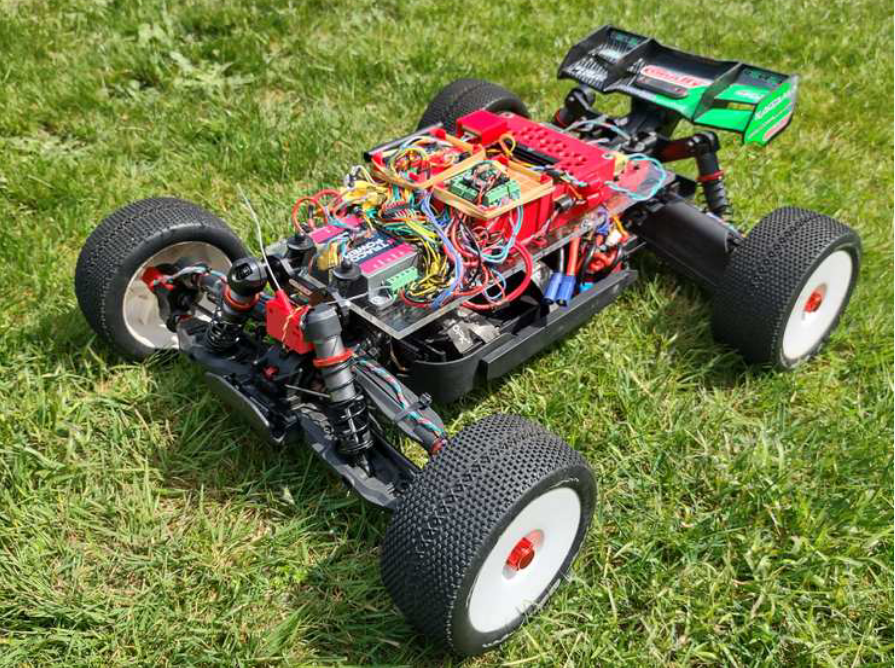
\includegraphics[width=\columnwidth]{images/truggysense_v1_assembly.png}
	\caption{The original TruggySense assembly~\cite{Elsermans2025}.}
	\label{fig:truggysense_v1_assembly}
\end{figure}

\section{Hardware architecture}
\ParagraphSeperator
The original TruggySense utilizes the existing Team Corally Kagama 1/8 RCV platform as a basis, on which both a High Level Controller (HLC) and Low Level Controller (LLC) are placed.
Additionally, numerous sensors and actuators were attached, which could reliably acquire data at high speeds whilst controlling the existing modules of the platform.
These actuators and sensors communicate with the LLC (as seen in Fig.~\ref{fig:truggysense_v2_hardware_architecture}); while the HLC communicates with both LiDAR and RADAR modules\footnote{All implementations regarding the HLC are part of a separate thesis, and thus are not implemented.}.

\begin{figure}[!t]
	\centering
	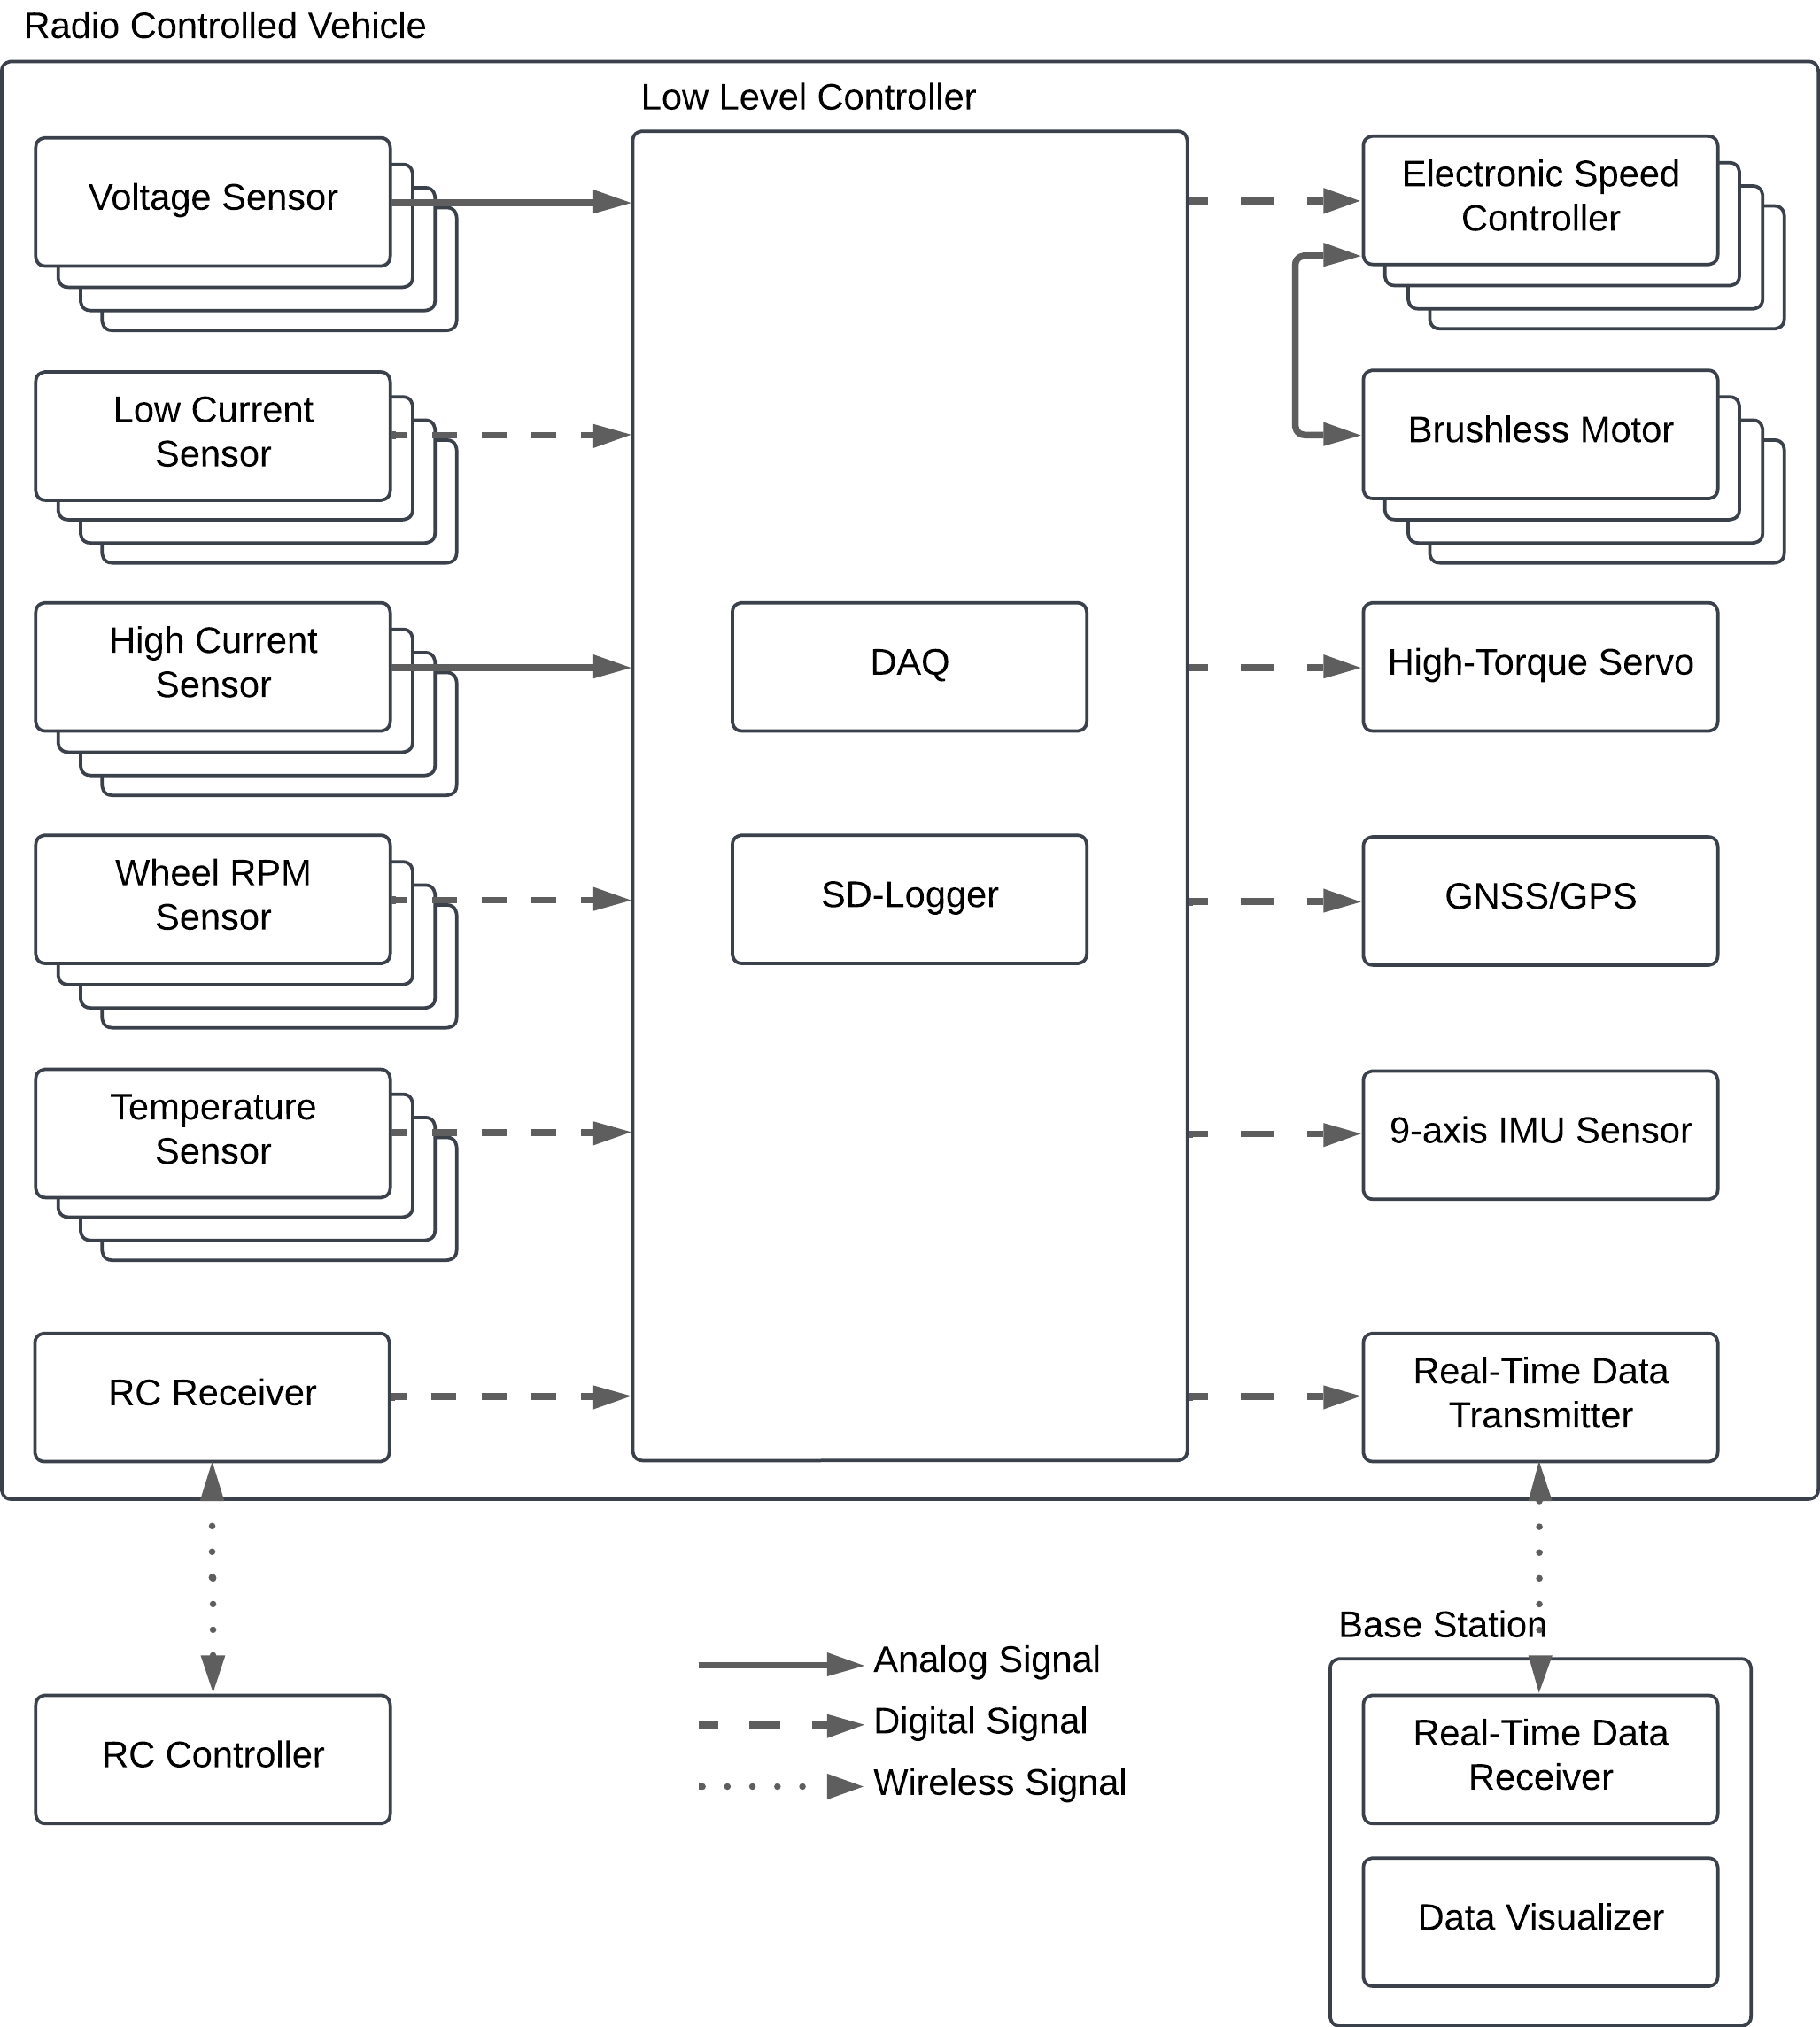
\includegraphics[width=\columnwidth]{images/hardware_architecture/hardware_architecture.png}
	\caption{
		An abstract block diagram that represents the TruggySense V2 hardware architecture. 
		This depicts the LLC as the DAQ, gathering data from all the sensors, while controlling the peripherals of the RCV unit.
	}
	\label{fig:truggysense_v2_hardware_architecture}
\end{figure}

\ParagraphSeperator
Fig.~\ref{fig:truggysense_v2_below_base_plate_assembly} displays the components that were mounted to the base of the Kagama frame.
The only modification made, compared to the first version of the TruggySense (TruggySense V1), is the replacement of temperature sensors.

\begin{figure}[!t]
	\centering
	% https://imageonline.io/add-arrow/
	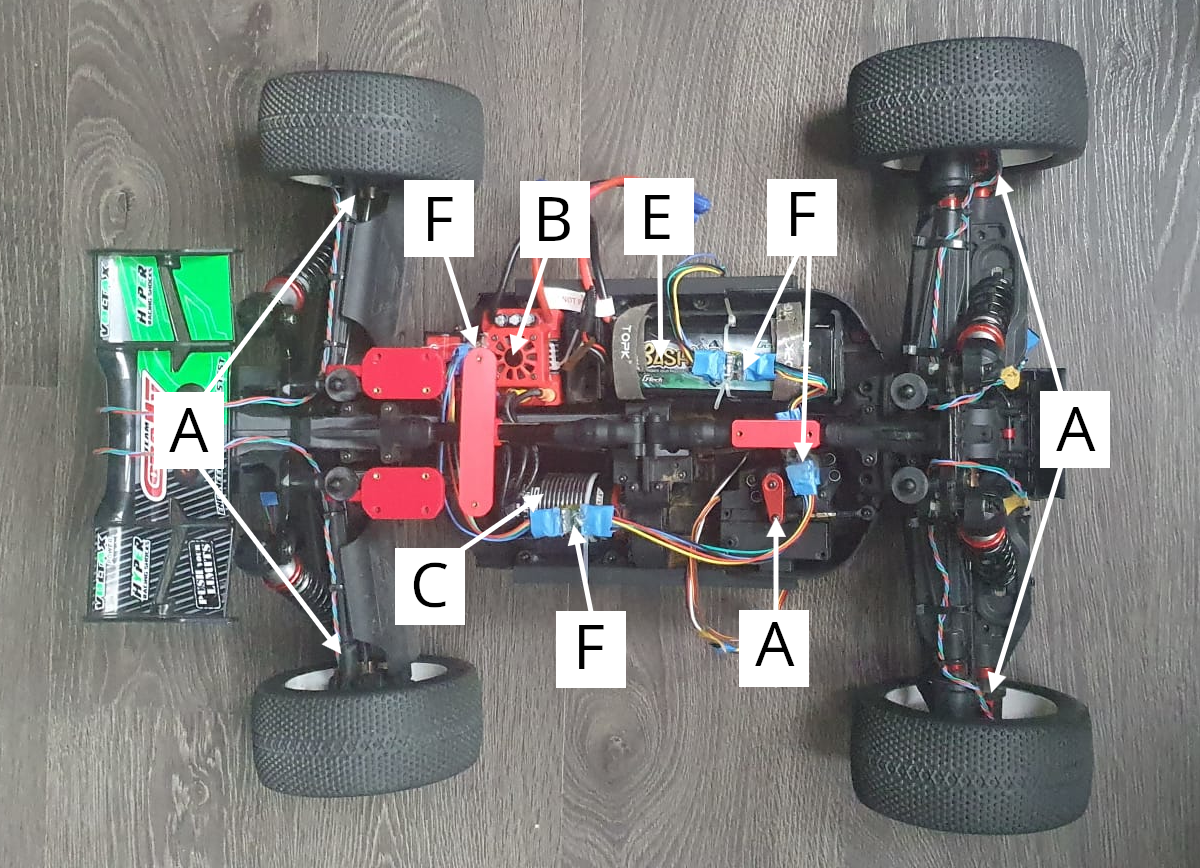
\includegraphics[width=0.378\textwidth]{images/hardware_architecture/car_bottom_indication.png}
	\caption{
		The hardware layout secured to the chassis of the Corally Kagama, without the base plate mounted, with:
		(A) The wheel encoders,
		(B) The ESC that controls the motor, provided by the Kagama RCV,
		(C) The brushless motor, provided by the Kagama RCV,
		(D) The steering servo,
		(E) The battery pack,
		(F) Various temperature sensors, on a custom-made PCB, daisy-chained together.
	}
	\label{fig:truggysense_v2_below_base_plate_assembly}
\end{figure}

\ParagraphSeperator
Fig.~\ref{fig:truggysense_v2_above_base_plate_assembly} shows the components that were mounted onto the base plate, which in turn is secured to the Kagama frame.
Multiple alterations have been made, compared to the TruggySense V1, including: 
(Fig.~\ref{fig:truggysense_v2_above_base_plate_assembly}.D) The 5V DC-DC converter being replaced by its 40W counterpart, due to the HLC demanding 3A under load;
(Fig.~\ref{fig:truggysense_v2_above_base_plate_assembly}.E) The supply board being separated from the logic board;
(Fig.~\ref{fig:truggysense_v2_above_base_plate_assembly}.H) The GPS being replaced\footnote{The new module was not intended to be used by the prototype. Since there was no connector nor mounting holes provided on the logic board, a separate casing was printed and mounted to the HLC.}.
													        Both the old and new GPS modules are u-blox modules that utilize NMEA-0183 messages\footnote{NMEA-0183 is a serial protocol that works in simplex mode~\cite{Langley1995}.}, thus the new module should be compatible with the old code;
(Fig.~\ref{fig:truggysense_v2_above_base_plate_assembly}.N) A cooling fan being added, due to the HLC significantly heating up, even when not under load;
(Fig.~\ref{fig:truggysense_v2_logic_prototype}.B) The low-Ampere sensors being replaced by their Inter-Integrated Circuit (I2C)\footnote{I2C is a two-wire serial communication protocol using a serial data line (SDA) and a serial clock line (SCL), to allow multiple devices to communicate over the same bus~\cite{Wu2022}.} counterpart.
												  This adds the possibility of redundancy, since the I2C variant allows up to 16 addresses on the same bus, compared to the old module that needs an Analog-to-Digital Conversion (ADC) pin for each module.

\begin{figure}[!t]
    \centering
	% https://imageonline.io/add-arrow/
	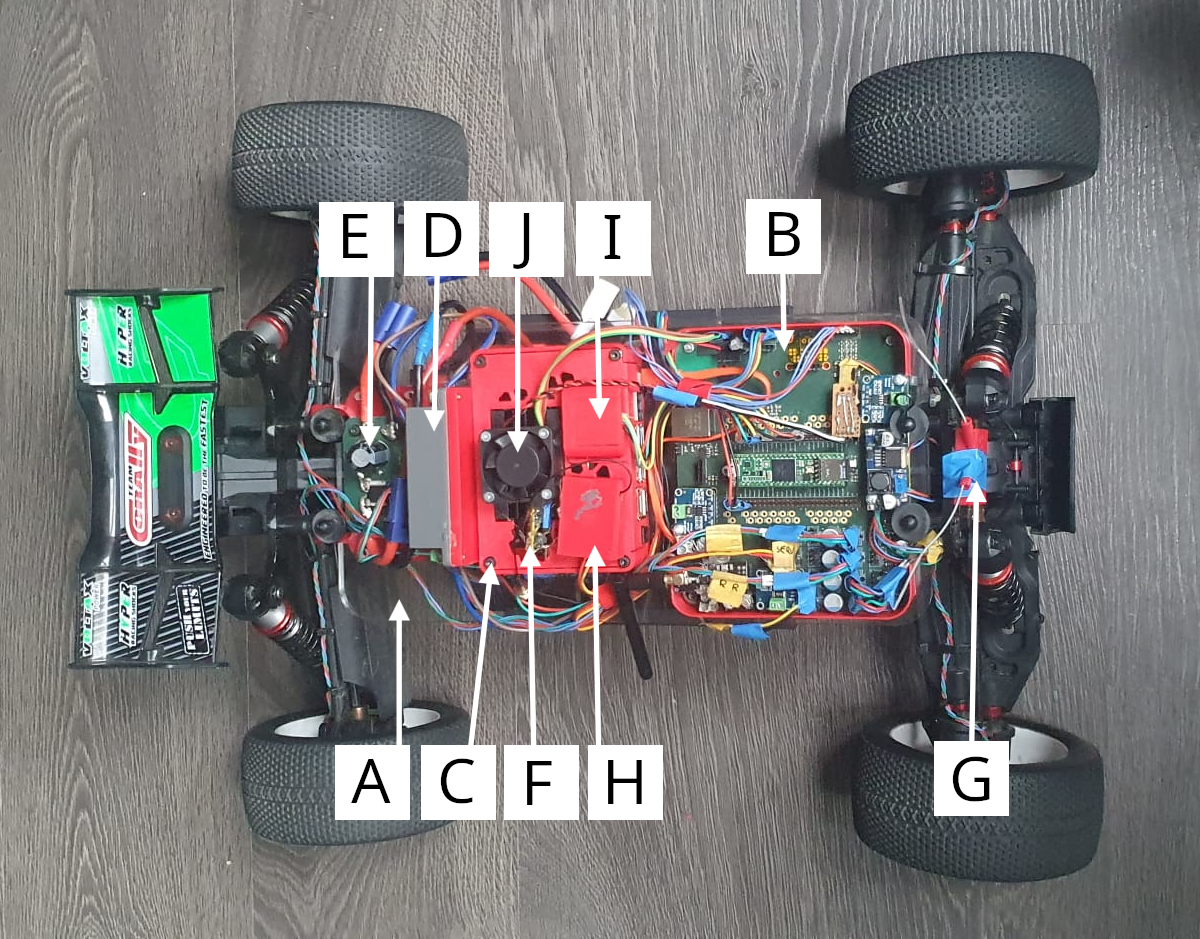
\includegraphics[width=0.378\textwidth]{images/hardware_architecture/car_middle_indication.png}
    \caption{
		The hardware layout mounted on top of the chassis of the Corally Kagama, utilizing the base plate, with:
		(A) The mounting plate,
		(B) The logic board,
		(C) The HLC,
		(D) The TMDC 40-2411 5V DC-DC 8A converter,
		(E) The supply board,
		(F) The dedicated temperature sensor for the HLC,
		(G) A FlySky X6B, used as the receiver for the remote,
		(H) The GNSS/GPS,
		(I) The 9-DOF IMU unit,
		(J) A 40×40mm fan, used to cool the HLC.
	}
	\label{fig:truggysense_v2_above_base_plate_assembly}
\end{figure}

\ParagraphSeperator
Fig.~\ref{fig:truggysense_v2_cover_assembly} displays the components that were attached to the lid of the Kagama.
The GPS antenna is placed on top of the lid to improve the signal strength (Fig.~\ref{fig:truggysense_v2_cover_assembly}.A).

\begin{figure}[!t]
	\centering
	% https://imageonline.io/add-arrow/
	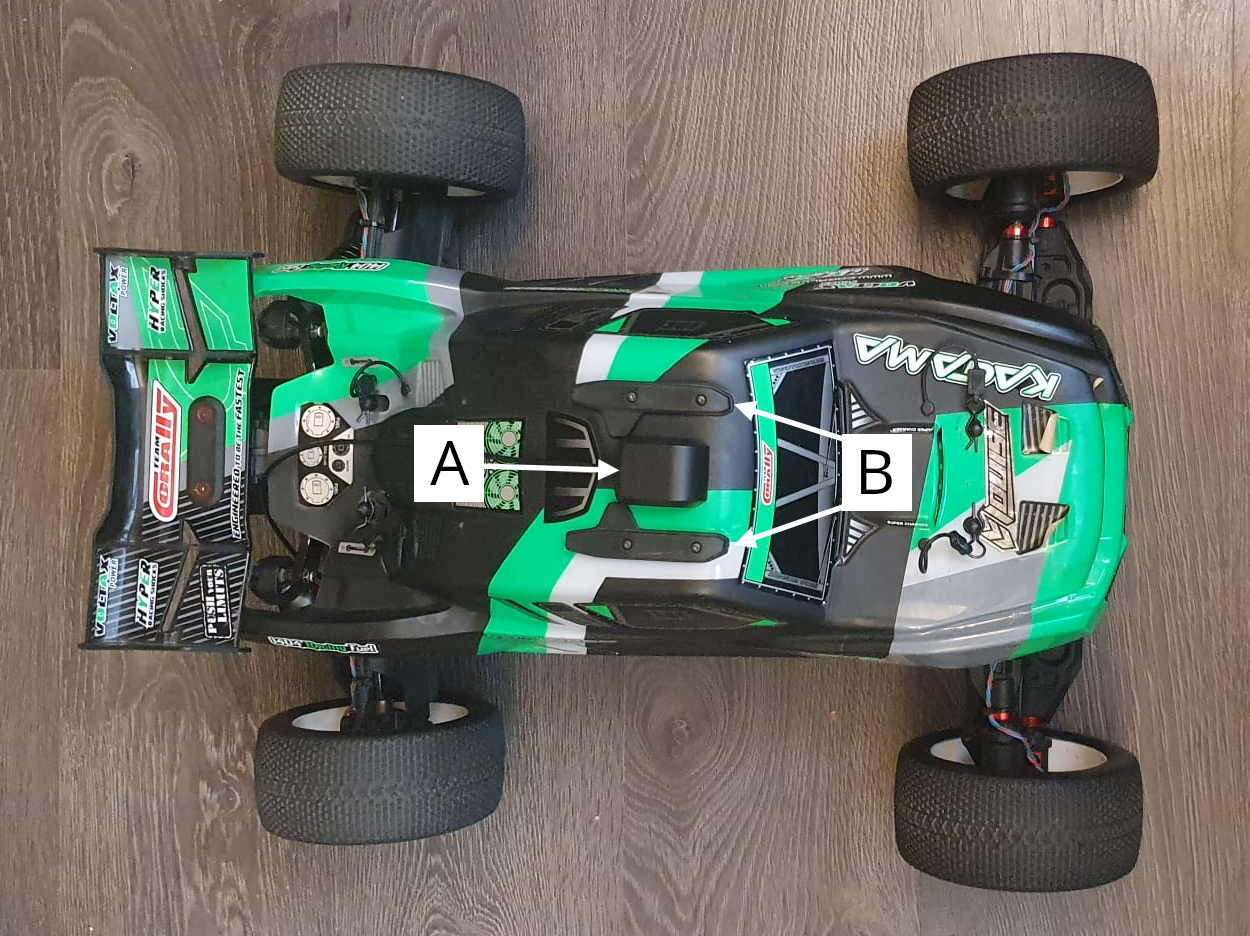
\includegraphics[width=0.378\textwidth]{images/hardware_architecture/car_top_indication.png}
	\caption{
		The hardware layout attached to the cover of the Corally Kagama, with:
		(A) The GPS antenna, attached using magnets below the cover,
		(B) Mounting brackets that hold the reflector, a folded piece of aluminum foil, to the inside of the roof of the cover.
	}
	\label{fig:truggysense_v2_cover_assembly}
\end{figure}

\subsection{PCB configuration}
\ParagraphSeperator
There are three custom-made PCBs used in this project: The logic board (Fig.~\ref{fig:truggysense_v2_logic_prototype}), the supply board (Fig.~\ref{fig:truggysense_v2_supply_prototype}), and the temperature sensor board (Fig.~\ref{fig:truggysense_v2_temperature_prototype}).
To reduce the assembly complexity, almost all modules and components are mounted directly onto the logic board, except for when this is not possible or logical, such as with the ESC, resulting in a connector being provided on the logic board.
Thus, justifying why the temperature sensors need their own PCB, since they must be affixed to their respective modules or components.

\ParagraphSeperator
The supply board is disconnected from the logic board to reduce the noise generated by the return current of the motor. 
A TMDC 40-2411 is placed between them, providing over-voltage protection and mitigating the effects of voltage and current fluctuations caused by battery discharge. 
Additionally, it offers short-circuit protection by limiting the output upon detection of a short circuit. 
Nevertheless, reverse polarity protection cannot be confirmed, since this claim is only made by third-party distributors and is absent from the official documentation.

\begin{figure}[!t]
    \centering
    % https://imageonline.io/add-arrow/
    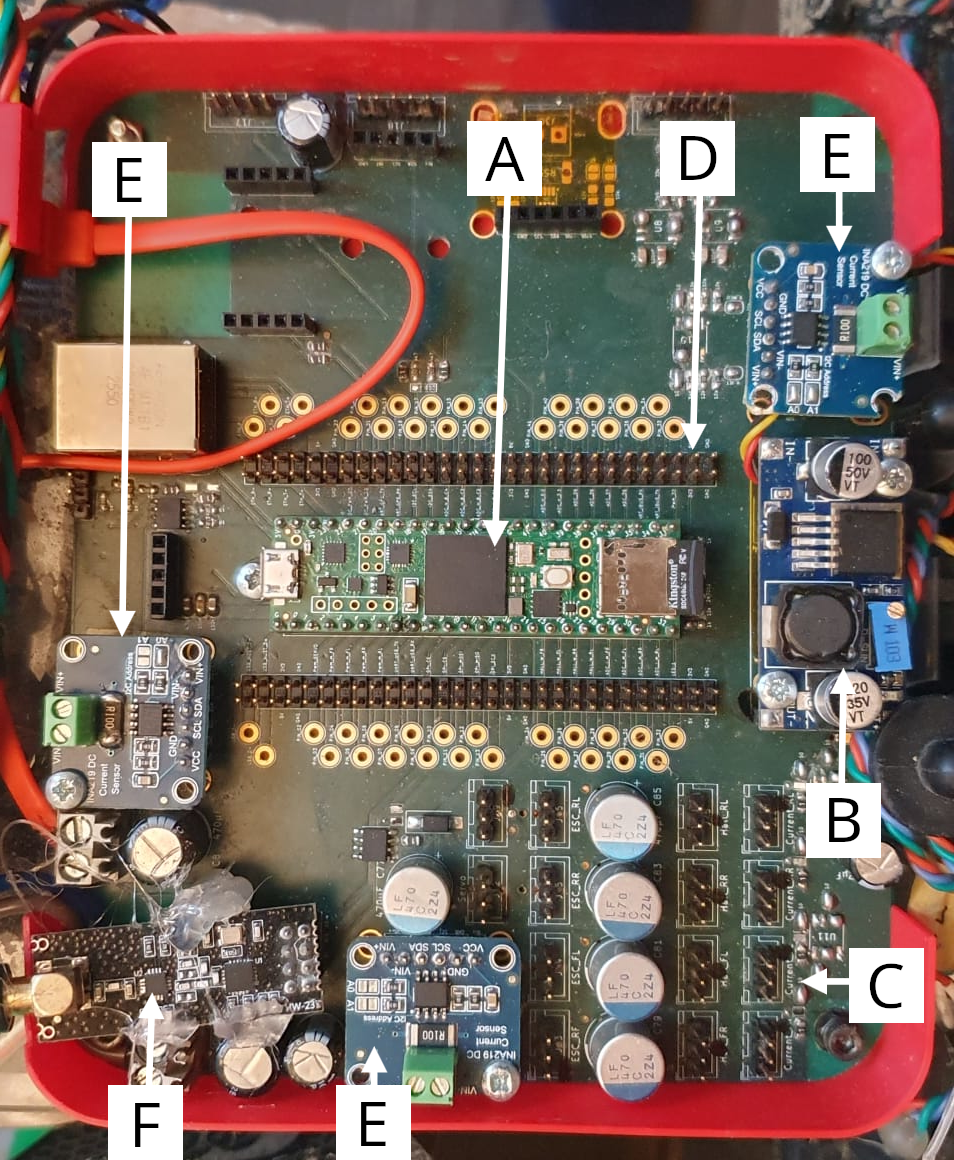
\includegraphics[width=0.378\textwidth]{images/hardware_architecture/logic_board_indication.png}
    \caption{
        The prototype logic board, with:
        (A) Teensy 4.1 as the LLC,
        (B) The LM2596\protect\stepcounter{footnote}\protect\footnotemark[\value{footnote}] 3.3V DC-DC step-down converter,
        (C) Connectors for IWD sensors and actuators, such as the high-ampere sensors, wheel encoders, and ESC for the motors --with four pin-headers for each--,
        (D) Double-rowed pin headers, connected directly to the pins of the LLC, for debugging and modifications if needed,
        (E) The INA219 low-Ampere sensors,
        (F) A nRF24L01\protect\stepcounter{footnote}\protect\footnotemark[\value{footnote}] module used for wireless data transmissions.
    }
    \label{fig:truggysense_v2_logic_prototype}
\end{figure}
\addtocounter{footnote}{-1}
\footnotetext{The original 3.3V DC-DC step-down converter was unidentifiable and was thus replaced. Note that this module will be replaced by an AMS1117-3.3 for a more stable supply.}
\stepcounter{footnote}
\footnotetext{nRF24L01 is a 2.4GHz chip that uses its own proprietary protocol. The original module, an E01-ML01DP5, made use of this chip. It was replaced since it was unavailable.}
\begin{figure}[!t]
	\centering
	% https://imageonline.io/add-arrow/
	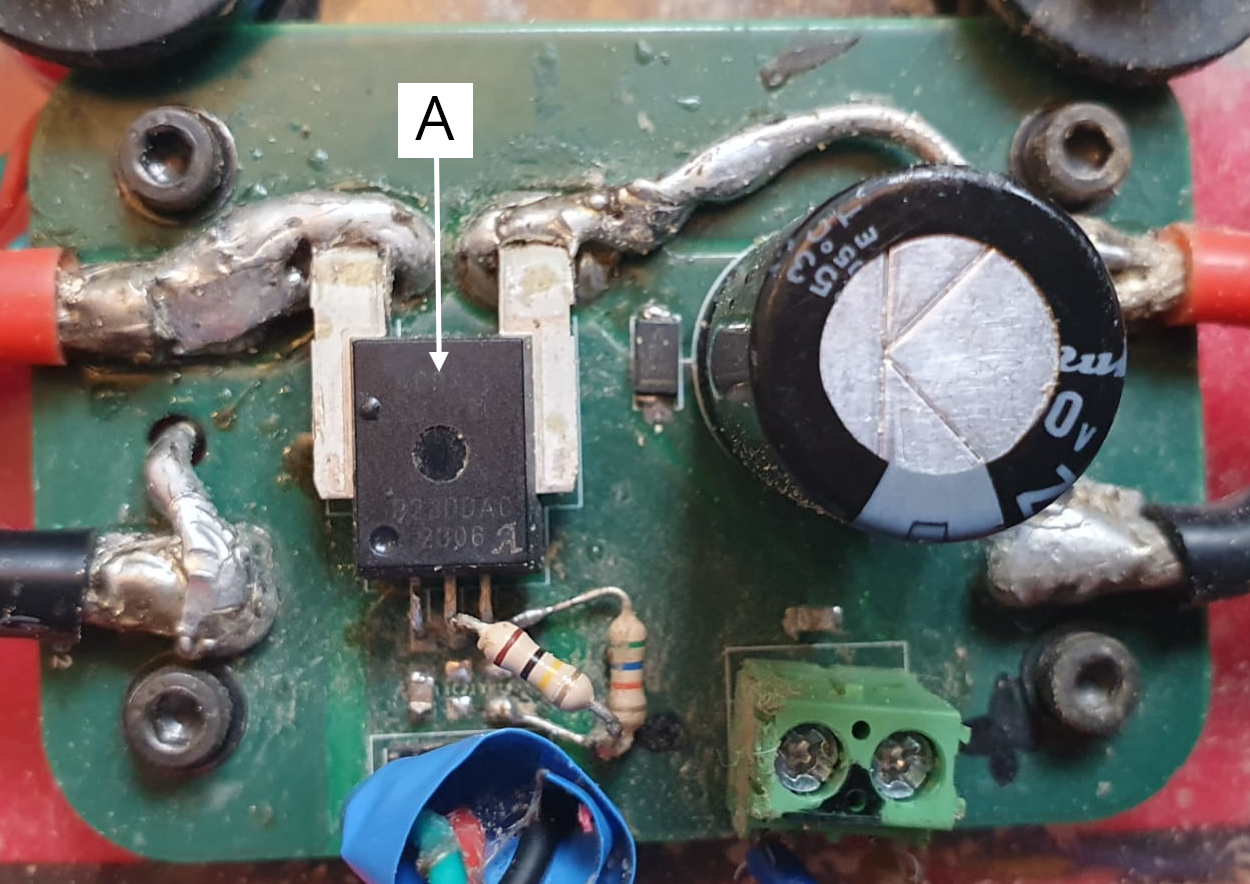
\includegraphics[height=0.378\columnwidth]{images/hardware_architecture/supply_board_indication.png}
	\caption{
		The prototype supply board, with:
		(A) ACS756 high ampere sensor.
	}
	\label{fig:truggysense_v2_supply_prototype}
\end{figure}
\begin{figure}[!t]
	\centering
	% https://imageonline.io/add-arrow/
	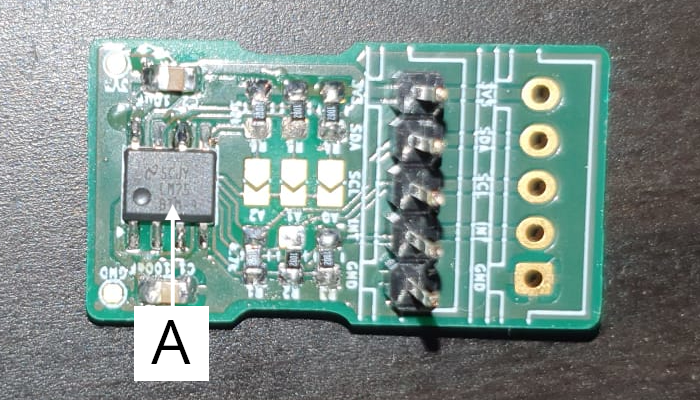
\includegraphics[width=0.378\columnwidth]{images/hardware_architecture/temperature_board_indication.png}
	\caption{
		The prototype temperature board, with:
		(A) LM75 temperature sensor.
	}
	\label{fig:truggysense_v2_temperature_prototype}
\end{figure}

\subsection{Board design}
\ParagraphSeperator
The prototype makes use of a four-layer topology:

\noindent\centerline{Signal | GND | Vcc | Signal}

\noindent The final PCBs make use of a six-layer topology\footnote{The design of the final PCB was completed (as shown in Fig.~\ref{fig:board_logic}). However, it was not manufactured or tested due to time constraints. All experiments were therefore conducted using the prototype.}: 

\noindent\centerline{Signal | GND | 3V3 | 5V | GND | Signal}

\noindent Using this method, every component has a ground reference in close proximity.
Furthermore, both source planes have an adjacent ground plane, forming a distributed capacitor, as the FR4 layer acts as a dielectric, filtering high-frequency noise.

\ParagraphSeperator
For the design rules, certain standard values are applied to the signal lines, low power lines, and high power lines (as displayed in Tab.~\ref{tab:pcb_design_rules}).
The trace widths $W$ are determined using equation~\ref{eq:track_width}~~\cite{Daems2023,IPC1998}.
\begin{align}
    \label{eq:track_current}
    I & = k \cdot \Delta T^{0.44} \cdot (W \cdot H)^{0.725} \\
    W & = \frac{1}{H} \cdot \left(\frac{I}{k \cdot \Delta T^{0.44}}\right)^{1/0.725}
\end{align}

Seeing as, the middle layers of the PCB stack are reserved for either supply or ground planes, the traces will be part of the outside layers, resulting in k = 0.048.
As for the temperature rise $\Delta T$ and track thickness $t$ (or $H$), the standard values of 10°C and 0.035mm or 1.378 mil (1oz. copper) are used, respectively.
\begin{align}
    \label{eq:track_width}
    W & = \frac{1}{1.378} \cdot \left(\frac{I}{0.048 \cdot 10^{0.44}}\right)^{\frac{1}{0.725}} \\
	  & = \frac{1}{1.378} \cdot \left(\frac{I}{0.1322}\right)^{1.379}
\end{align}

This also means that a track width of $\sim$0.45m would be needed to allow a current of 200A.
Thus, a solid copper wire, with a core surface of 2.5mm², was added to support the high current provided by the battery.

\ParagraphSeperator
As for the vias, these should be as small as possible, while having enough surface to support the current that will pass through them.
This is determined using equation~\ref{eq:via_current}\footnote{The intermediate steps of these equations are found in the appendix under equation~\ref{eq:proof_track_width} and equation~\ref{eq:proof_via_width}.}.
\begin{align}
    \label{eq:via_surface}
    A & = A_{hole} - A_{hole - copper} \\
	  & = \pi \cdot t \cdot (d_{hole} - t)
\end{align}

\noindent Substituting it into equation~\ref{eq:track_current}, results in:
\begin{align}
    d_{hole} & = t + \frac{1}{\pi \cdot t} \cdot \left(\frac{I}{k \cdot \Delta T^{0.44}}\right)^{\frac{1}{0.725}} \\
	\label{eq:via_current}
             & = 1.378 + 0.231 \cdot \left(\frac{I}{0.1322}\right)^{1.3793}
\end{align}

\noindent The pad diameter is set to twice the hole diameter, to ensure a good connection between the via and the layers.

\ParagraphSeperator
Finally, for spacing, a 0.13mm clearance should suffice for the signal and low power lines~\cite{Daems2023}.
As for the high power lines, a clearance of at least 1mm is implemented to ensure that the ground plane of the logic and supply boards can never connect to each other.

\begin{table*}[!t]
	\centering
	\caption{PCB Design Rules}
	\begin{tabular}{lcccccccc}
		\toprule
			Line type & \multicolumn{2}{c}{Power}   						& \multicolumn{2}{c}{Traces} 					     & \multicolumn{3}{c}{Vias}   						                             & Spacing \\
					  &	\scriptsize{Voltage (V)} & \scriptsize{Current (A)} & \scriptsize{Width (mil)} & \scriptsize{Width (mm)} & \scriptsize{Hole (mil)}  & \scriptsize{Hole (mm)} & \scriptsize{Diameter (mm)} & \scriptsize{Clearance (mm)} \\
		\cmidrule(lr){2-3}\cmidrule(lr){4-5}\cmidrule(lr){6-8}\cmidrule(lr){9-9}
			Signal     & \textless 5.1  & \textless 0.1 & 0.494 & 0.0125 & 1.535 & 0.039 & 0.078 & 0.13 \\
			Low power  & \textless 5.1  & \textless 2   & 30.76 & 0.7814 & 11.17 & 0.284 & 0.568 & 0.26 \\
			High power & \textless 16.8 & \textless 200 & 17647 & 448.22 & 5619  & 142.7 & 285.4 & 1.3  \\
		\bottomrule
	\end{tabular}
	\label{tab:pcb_design_rules}
\end{table*}

\subsection{IWD support}
\ParagraphSeperator
One of the goals of the TruggySense second version (TruggySense V2) is to support IWD.
For this purpose, research towards custom-made motors has not been started, but is still ongoing.
Thus, support for both the old Corally Kagama system --containing the Corally Kuron 825 motor and Corally Torox 185 ESC--, and the new four motor system has to be included (Fig.~\ref{fig:truggysense_v2_above_base_plate_assembly}.J).

\ParagraphSeperator
The project towards these custom motors is currently developing direct drive motors\footnote{Direct drive motors are motors that are inserted into the socket of each wheel, eliminating the need for a gearbox.}.
This leads to the possibility of the current wheel encoders and motor temperature sensors becoming redundant, and a need for them to be integrated into the motor itself.
Compatibility for these new sensors is provided by the open pin headers (Fig.~\ref{fig:truggysense_v2_above_base_plate_assembly}.K), which are connected directly to pins of the LLC.

\subsection{Temperature sensor}
\ParagraphSeperator
When the system is operating, certain components can draw up to 200A under load, which may cause overheating and the failure of the component.
A Li-Po Battery must provide these peak currents, possibly overheating itself.
Therefore, monitoring these components is critical.

\ParagraphSeperator
Previously, this was done via DS18B20+, but this module is replaced by the LM75, due to its lower cost.
However, this comes with two drawbacks: fewer devices on the same bus, and reduced accuracy, going from ±0.5°C to ±2°C, though this should not affect the performance of the TruggySense V2.
The LM75 makes use of the I2C protocol, with each sensor having its own identifier, called an address.
These addresses are assigned by connecting the three address pins to either ground or its supply, leaving the module with eight usable addresses, compared to the 64-bit identifier of the DS18B20+.
Though, by adding an expansion module such as the LTC4316, the number of unique addresses for the LM75 can be increased to 32.

\subsection{Motion sensor}
\ParagraphSeperator
Whilst driving, some of the most critical metrics are the direction, acceleration, and velocity of the vehicle.
Currently, this is sensed and computed by a BNO085, a nine-degree-of-freedom (9-DoF) Inertial Measurement Unit (IMU).
Though a replacement was planned, being the PIM448 module, which integrates the ICM20498 chip with an integrated AK09916 magnetometer.
Unlike the BNO048, the PIM448 could not independently compute roll, pitch, and yaw; it could only provide raw rotational acceleration and magnetic field data.
To generate the orientation angles, a Mahony filter was implemented on the LLC, providing similar readings to the BNO085.

\ParagraphSeperator
Ultimately, the PIM448 was not integrated into the current system, due to the magnetometer not initializing while the battery is plugged in.
The cause for this are the minor noise artifacts, originating from the supply board, that are able to pass through the 5V DC-DC converter (as illustrated by Fig.~\ref{fig:supply_noise}), causing a brown-out in the AK09916.
Thus, the BNO085 was reused as the IMU and mounted to the top of the HLC, since there was no connector provided on the logic board\footnote{Both the BNO085 and PIM448 have been implemented in the completed design of the logic board.}.

\subsection{Global positioning}
\ParagraphSeperator
While the measurements of the DAQ verify wether the system is operational, the GPS enables the validation of this data by comparing it to the real world, making it a crucial component.
For these purposes, a GY-NEO6M module was used, instead of the M10FD, due to the original being unavailable.
Both are u-block GPS modules, and thus make use of UART, with a standard baud rate of 9600 --corresponding to a transmission speed of 9600 bits per second (bps)-- and the 8N1\footnote{UART always starts with one start-bit, and the 8N1 notation indicates the following: '8' indicates eight data-bits are send per frame, 'N' indicates that no parity-bit is used, and '1' indicates one stop-bit is used.} configuration.
Meaning that every byte needs 10 bits to be send, resulting in a transmission speed of 960 bytes per second (Bps) or a byte period of $\sim$1.04ms.
The scheduler of the firmware utilizes multiple interrupts, some repeating every millisecond, causing the data to become unintelligible.

\ParagraphSeperator
To solve this problem, the UART baud rate needs to be increased.
Most u-blox GPS modules allow a baud rate of up to 115200, resulting in a byte period of $\sim$86.81µs.
Each of the u-block modules could be flashed to these higher transmission speeds, using a proprietary tool, but only the M10FD stores this after power has been lost.
Thus, the firmware will have to initialize the module at a baud rate of 9600 and increase it to 115200 before the scheduler is initiated.

\subsection{Data logging}
\ParagraphSeperator
To study the performance of the ADAS, data is logged both on an SD card and via wireless transmission.
To verify the real-time performance of the DAQ, an nRF24L01 was utilized for that wireless connection.
This is a 2.4GHz module that uses its own proprietary protocol.

\ParagraphSeperator
It is crucial that a variant with a built-in Power Amplifier (PA) and Low Noise Filter (NLA) circuit is used, 
since the PA circuit could improve the signal up to 20dBm on the transmitter side, 
while the LNA circuit is capable of improving the sensitivity of the receiver up to 10dB.
This results in a sensitivity of -104dBm in 250kbps mode --the data rate could be increased at the cost of sensitivity-- resulting in a range of around 1.5km in open-air.

\section{Experiment setup and Results}
As demonstrated by the TruggySense V1, the system is designed to verify and validate the ADAS under various off-road conditions.
To prove this, four experiments were performed on a predefined path (Fig.~\ref{fig:track}): (1) Slow driving, (2) Fast driving, (3) Failure detection, and (4) Crash detection.
Experiments (1) and (2) have proven that the system is able to detect the characteristics of the environment, using data pertaining to the condition of the vehicle, while experiments (3) and (4) were, in turn, able to demonstrate that the DAQ could sense malfunctions.

\begin{figure}[!t]
	\centering
	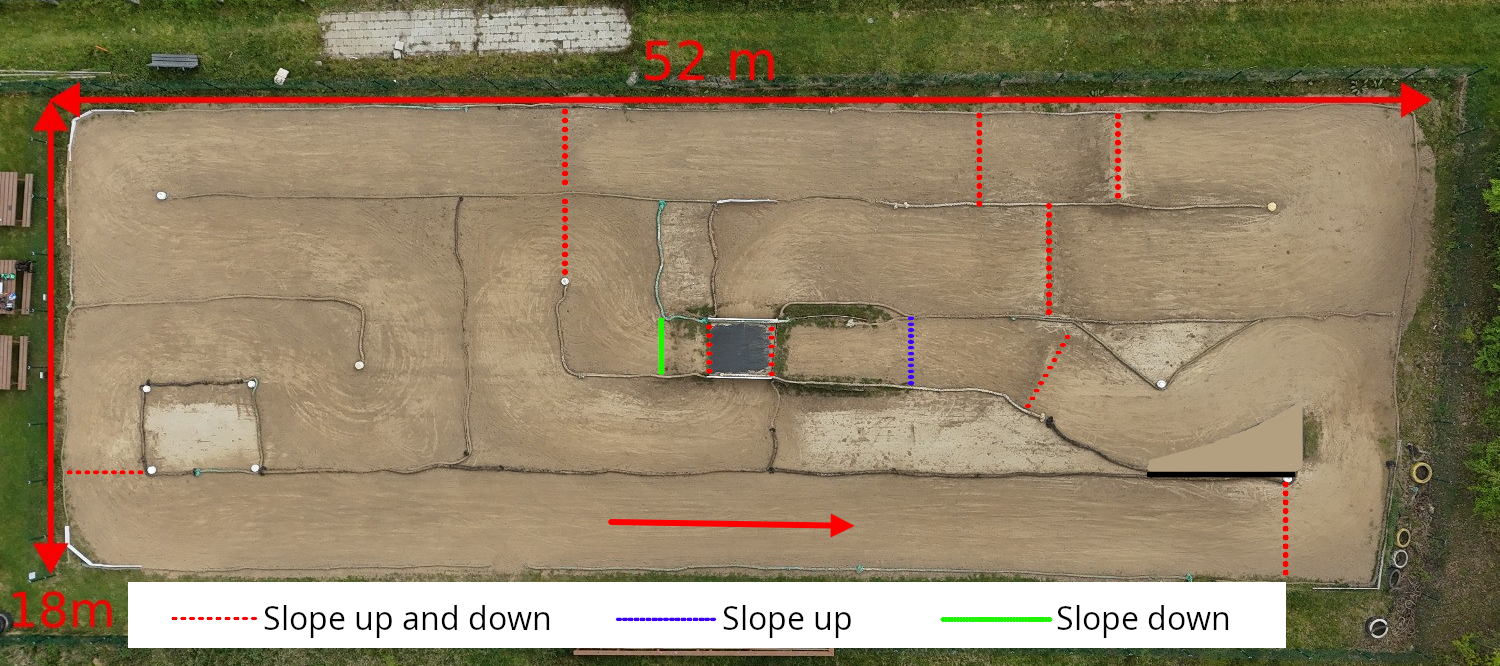
\includegraphics[width=\columnwidth]{images/experiments/track_indication.png}
	\caption{
		The experiment trajectory maintained by RC Racing Fun Bornem, located at Bornem, Antwerp, Belgium.
		There are different terrain features embedded into the track, such as hills, uneven terrain, a tunnel, sharp corners, and straight paths, making it a challenge to navigate this track~\cite{Elsermans2025}.
		Note that the track has been slightly altered compared to the TruggySense V1 experiments, with the sand of the elevated platform in the bottom right corner being moved to steepen the hills located on the top lane.
	}
	\label{fig:track}
\end{figure}

\ParagraphSeperator
As for the experiments, only the first and second are executed and discussed by the current system, since they display whether the system is operating similarly to its predecessor.
The first experiment, "Slow driving" is meant to form a baseline, during which the system will operate at its lowest possible settings.
The second "Fast driving" is meant to demonstrate the system under strain.
Besides this, the stability and accuracy of the DAQ will be evaluated by performing stationary experiments.

\subsection{Slow driving over the track} 
\ParagraphSeperator
During this experiment, the RCV is driven slowly and at a constant speed.
As demonstrated in Fig.~\ref{fig:exp1_fig1}, the position data-points clearly correlate with the route taken on the track.

\begin{figure}[!t]
	\centering
	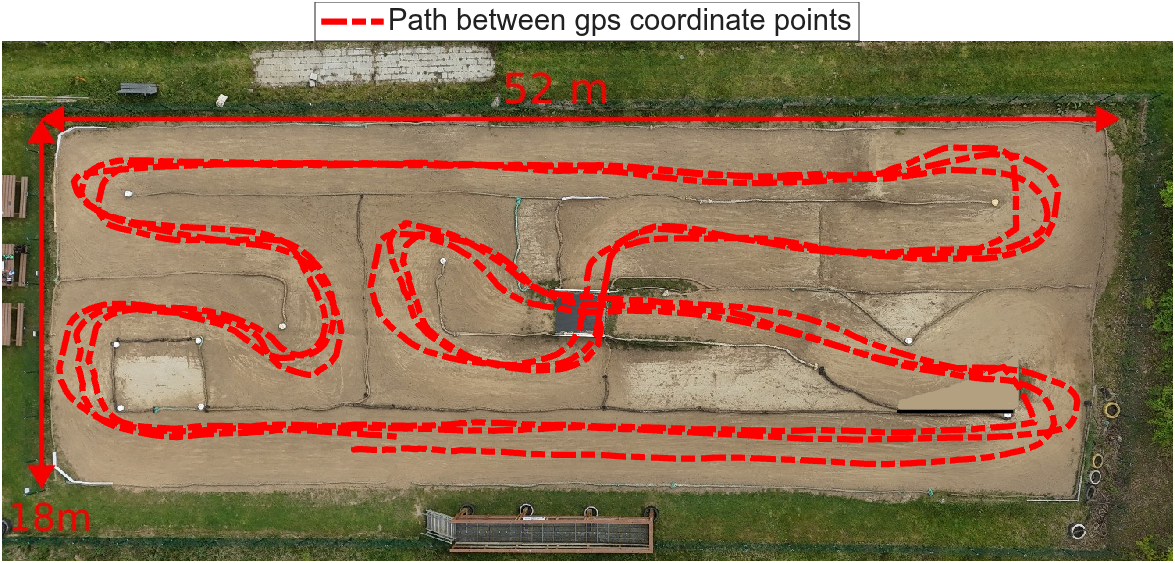
\includegraphics[width=\columnwidth]{images/experiments/exp1_fig1.png}
	\caption{
		GPS reference of the TruggySense V2, during the "Slow driving" experiment.
	}
	\label{fig:exp1_fig1}
\end{figure}

\ParagraphSeperator
Fig.~\ref{fig:exp1_fig3_v2} reveals that terrain variations, such as divots, ridges, and slopes, are reflected in the pitch angle: a positive value corresponds to an incline, while a negative value indicates a decline. 
These results are consistent with those of the TruggySense V1 (Fig.~\ref{fig:exp1_fig3_v1}), and further capture track changes, including the displacement of sand from the elevated platform in the bottom-right corner toward the upper lane.

\begin{figure}[!t]
	\centering
	\subfloat[Pitch angle of the TruggySense V1.]{
		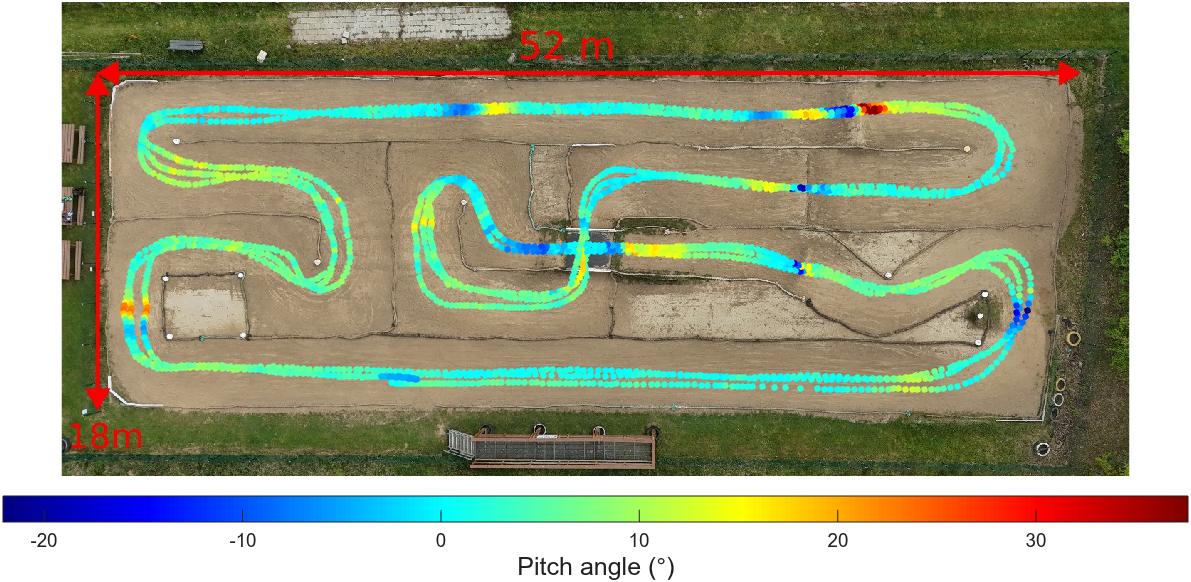
\includegraphics[width=\columnwidth]{images/experiments/exp1_fig3_v1.png}
		\label{fig:exp1_fig3_v1}
	} \hfil
	\subfloat[Pitch angle of the TruggySense V2.]{
		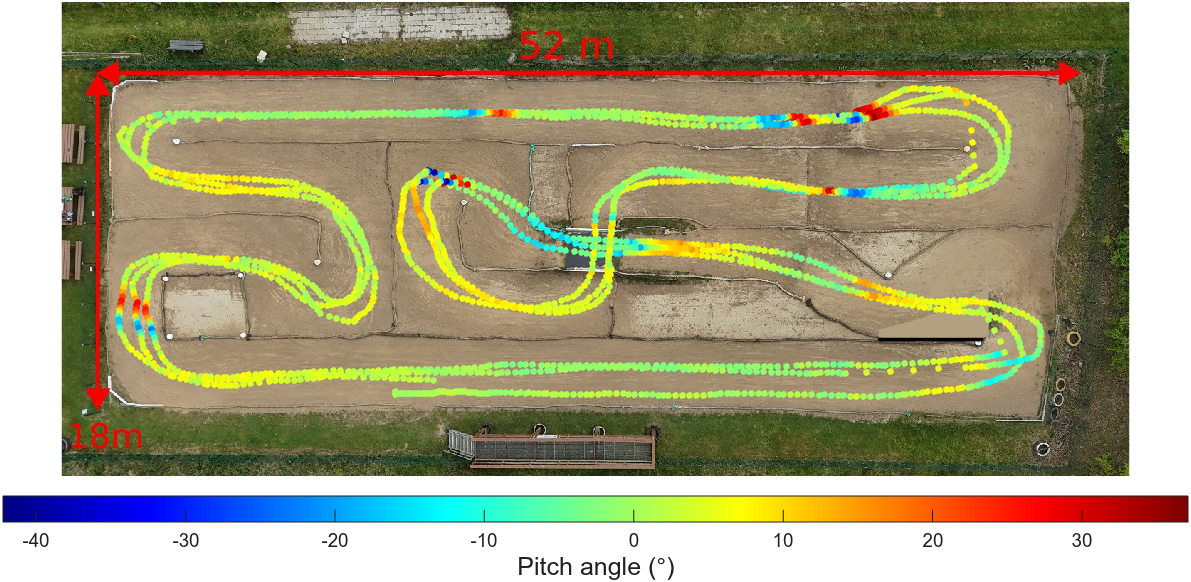
\includegraphics[width=\columnwidth]{images/experiments/exp1_fig3_v2.png}
		\label{fig:exp1_fig3_v2}
	}
	\caption{Difference in pitch angle, during the "Slow driving" experiment.}
	\label{fig:exp1_fig3}
\end{figure}

\ParagraphSeperator
The RCV features three differentials, one at the front, rear, and middle, enabling the wheels to rotate at different speeds whilst turning a corner.
Fig.~\ref{fig:exp1_fig3_v2} demonstrates that the direction of a turn can be discerned from the data gathered by the DAQ: a negative value corresponds to a clockwise turn, while a positive value indicates a counterclockwise turn.
This is consistent with the TruggySense V1 results presented in Fig.~\ref{fig:exp1_fig3_v1}.

\begin{figure}[!t]
	\centering
	\subfloat[Normalized wheel speed difference of the TruggySense V1. Note that the data was processed by computing the range (max $-$ min) across all four wheels simultaneously.]{
		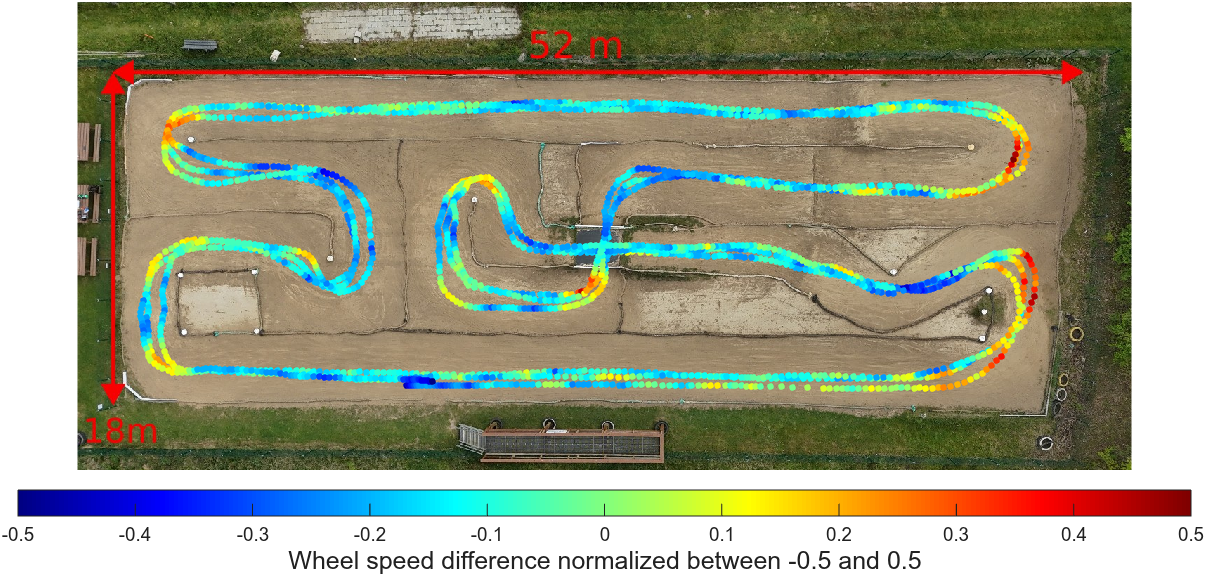
\includegraphics[width=\columnwidth]{images/experiments/exp1_fig2_v1.png}
		\label{fig:exp1_fig2_v1}
	} \hfil
	\subfloat[Normalized wheel speed difference of the TruggySense V2. Note that the data was processed by grouping the left wheels and right wheels together, and subtracting the mean of the left group from the mean of the right group.]{
		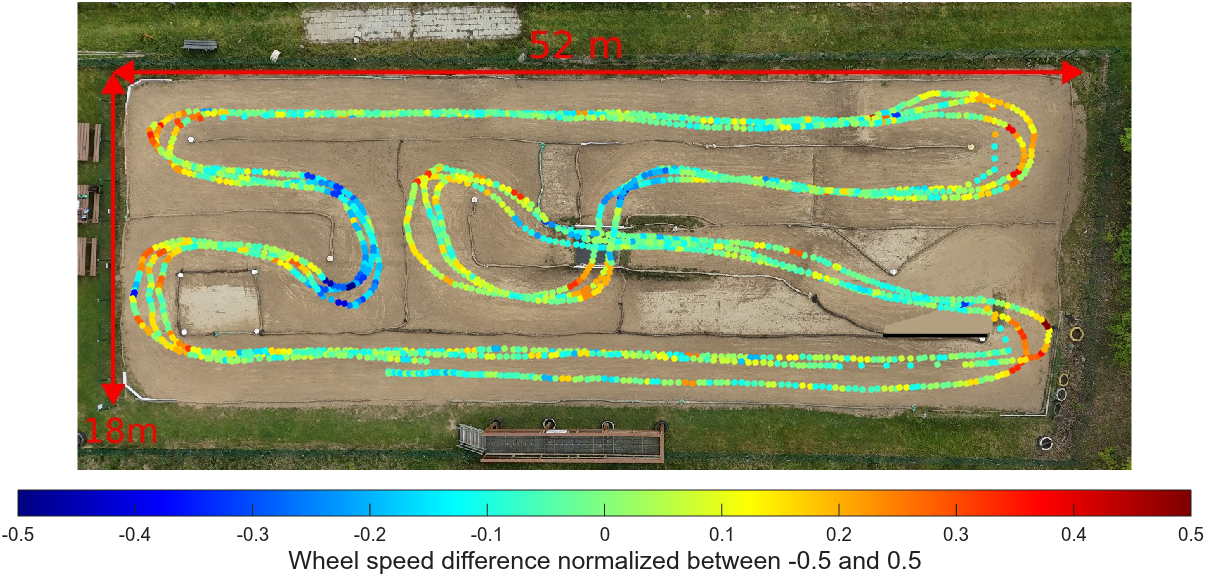
\includegraphics[width=\columnwidth]{images/experiments/exp1_fig2_v2.png}
		\label{fig:exp1_fig2_v2}
	}
	\caption{Difference in left and right wheel speeds, during the "Slow driving" experiment.}
	\label{fig:exp1_fig2}
\end{figure}


\ParagraphSeperator
Due to the nature of this experiment, the RCV has a lower power consumption and, in turn, reduced heating.
Fig.~\ref{fig:exp1_fig4} illustrates that the temperatures of the motor ESC $ t_{esc_{1}} $ and $ t_{m_{1}} $ both increased after prolonged usage, while battery pack $ t_{bp} $ and  steering servo $ t_{ss} $ maintained a steady temperature.

\begin{figure}[!t]
	\centering
	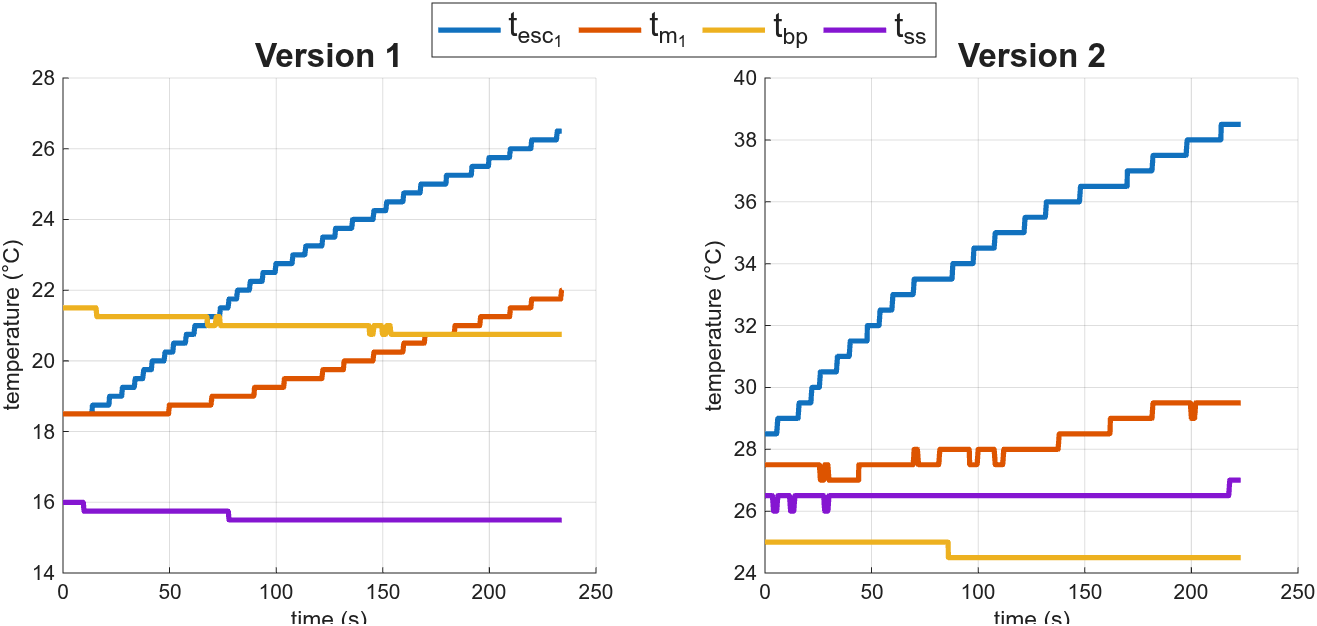
\includegraphics[width=\columnwidth]{images/experiments/exp1_fig4.png}
	\caption{
		Temperature comparison of the active components between the TruggySense V1 and V2 during the "Slow driving" experiment.
		The following components where measured: $esc_{1}$ = ESC, $m_{1}$ = Motor, $bp$ = Battery Pack, and $ss$ = Steering Servo.
	}
	\label{fig:exp1_fig4}
\end{figure}

\subsection{Fast driving over the track}
\ParagraphSeperator
During this experiment, the RCV was driven at a higher speed than during the previous experiment, with a throttle maintained at approximately twice the value as used previously.
The increase in speed leads to a wider spacing between the GPS data-points and greater wheel slip, as indicated by the steep inclines and declines in Fig.~\ref{fig:exp2_fig1_v2}.
These results are consistent with those of the TruggySense V1 (Fig.~\ref{fig:exp2_fig1_v2}).

\begin{figure}[!t]
	\centering
	\subfloat[Normalized wheel speed difference of the TruggySense V1.]{
		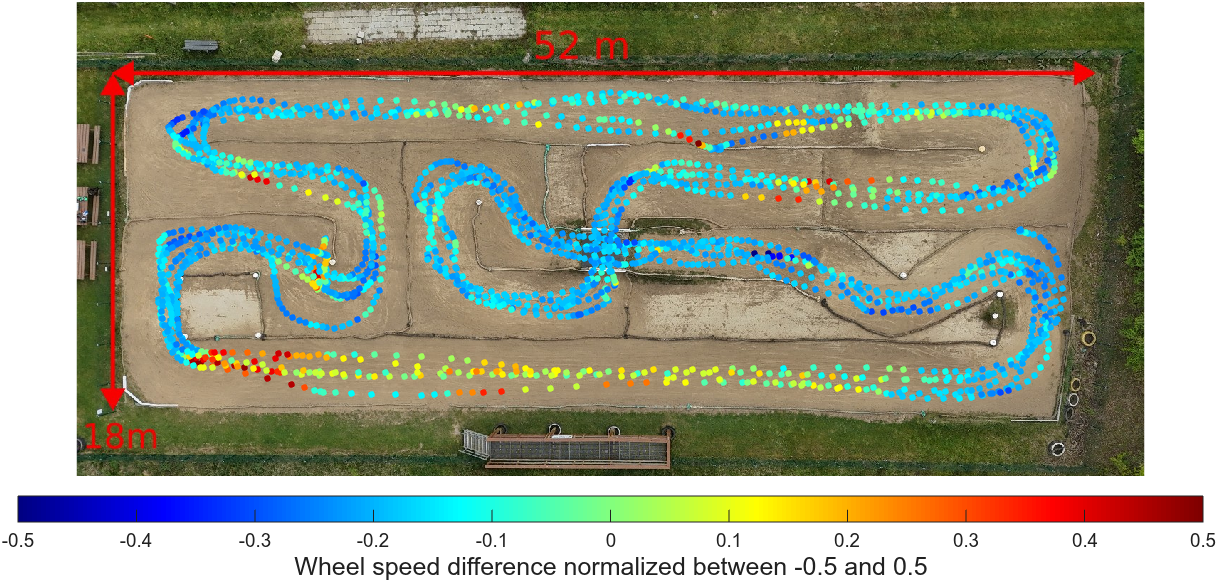
\includegraphics[width=\columnwidth]{images/experiments/exp2_fig1_v1.png}
		\label{fig:exp2_fig1_v1}
	} \hfil
	\subfloat[Normalized wheel speed difference of the TruggySense V2.]{
		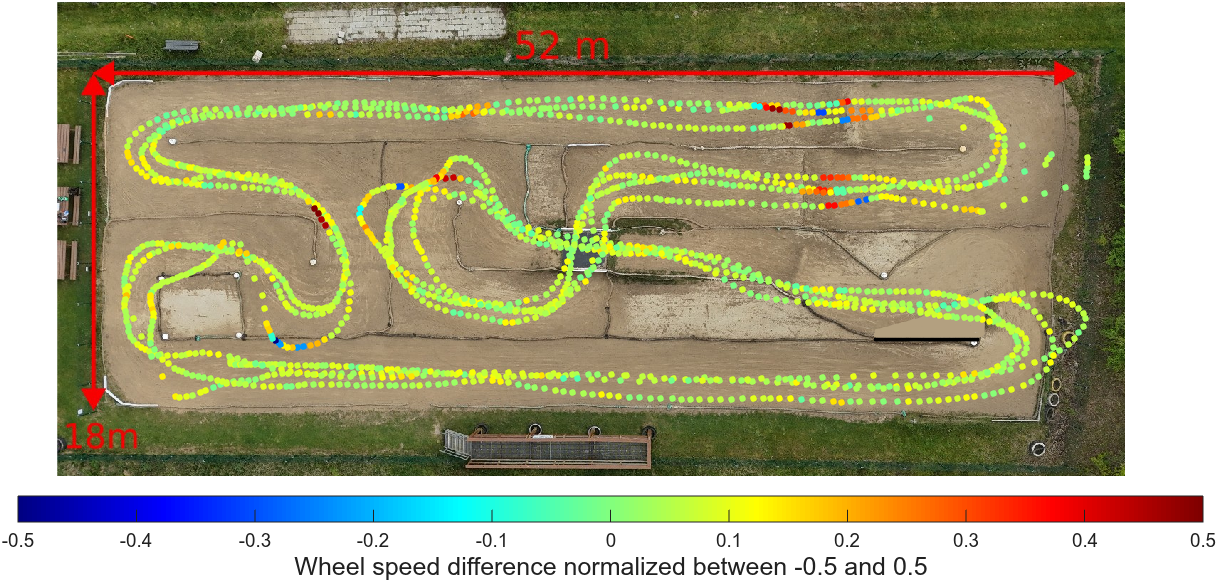
\includegraphics[width=\columnwidth]{images/experiments/exp2_fig1_v2.png}
		\label{fig:exp2_fig1_v2}
	}
	\caption{Difference in front and back wheel speeds, during the "Fast driving" experiment.}
	\label{fig:exp2_fig1}
\end{figure}

\ParagraphSeperator
Fig.~\ref{fig:exp2_fig2} compares the temperature difference of the ESC $ t^{f}_{esc_{1}} - t^{s}_{esc_{1}} $, motor $ t^{f}_{m_{1}} - t^{s}_{m_{1}} $ and battery pack $ t^{f}_{bp} - t^{s}_{bp} $, compared to previous experiment.
While there is a temperature increase, it is relatively low compared to the increase that was measured by the TruggySense V1.
This, in combination with the wider distances between GPS data points, suggests that the original tests were done at a higher speed.
Additionally, the change in sensor has introduced a clear reduction in accuracy.

\begin{figure}[!t]
	\centering
	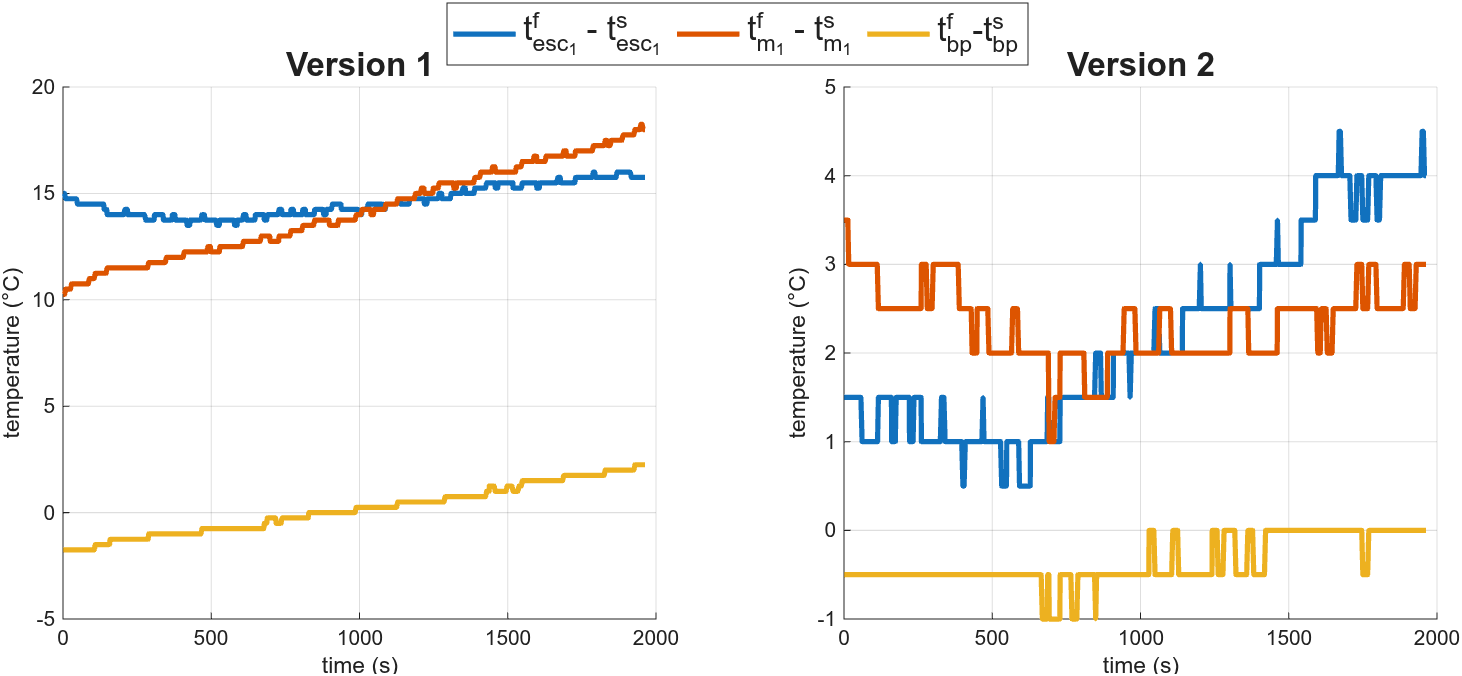
\includegraphics[width=\columnwidth]{images/experiments/exp2_fig2.png}
	\caption{
		Temperature difference between "Fast driving" and "Slow driving" experiments of the TruggySense V1 and V2.
		The following components where measured: $esc_{1}$ = ESC, $m_{1}$ = Motor, and $bp$ = Battery Pack.
	}
	\label{fig:exp2_fig2}
\end{figure}

\ParagraphSeperator
Under higher speeds, minor steering adjustments result in greater turns, which could destabilize the RCV.
However, Fig.~\ref{fig:exp2_fig4} suggests that this affects the TruggySense V2 less than the V1.
The difference might caused by more precise driver input, a lower operating speed compared to the original "Fast driving" experiment, or the recalibration of the neutral positions of the front wheels to reduce drift\footnote{Unlike the rear wheels, the front wheels are not perpendicular to each other. If they are not calibrated correctly, this could cause the vehicle to drift to one side.}.
Since the difference in speed was already inferred from Fig.~\ref{fig:exp2_fig1} and Fig.~\ref{fig:exp2_fig2}, the lower operating speed is the most likely reasoning.

\begin{figure}[!t]
	\centering
	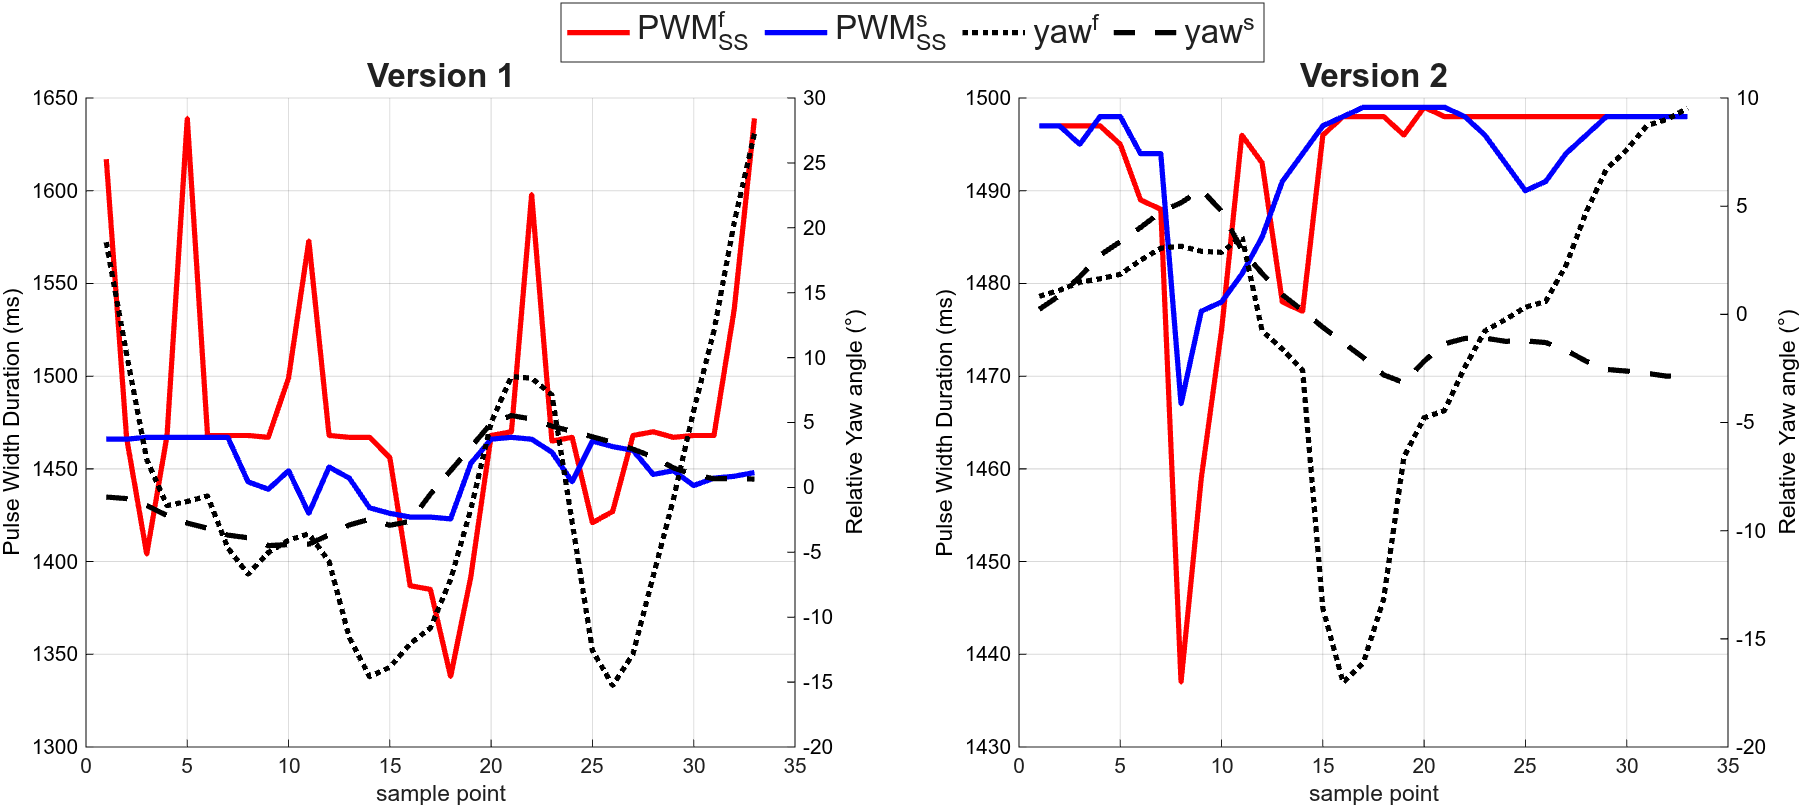
\includegraphics[width=\columnwidth]{images/experiments/exp2_fig4.png}
	\caption{
		Raw PWM values of the steering servo with yaw angles between "Fast driving" and "Slow driving" experiments of the TruggySense V1 and V2.
	}
	\label{fig:exp2_fig4}
\end{figure}

\subsection{Stability and accuracy of the DAQ}
\ParagraphSeperator
During these experiments, the system was placed upon an elevated platform with the wheels suspended in the air to permit free rotation.
As the majority of the "Slow driving" and "Fast driving" experiments rely on positioning, orientation angles, and wheel speed data, the accuracy of these sensors is evaluated in this section.

\ParagraphSeperator
Fig.~\ref{fig:exp_position} visualizes the accuracy of the positioning.
Using the Haversine formula~\cite{Robusto1957} --to convert a difference in latitude $\Delta\varphi$ and longitude $\Delta\lambda$ to meters (compared to the mean radius of the earth $R$)-- the distance between the center and the furthest point of each data is calculated (as presented in Tab.~\ref{tab:position_distance}).
\begin{align}
	a & = \sinsq\left(\frac{\Delta\varphi}{2}\right) + \cos{(\varphi_1)} \cos{(\varphi_2)} \sinsq\left(\frac{\Delta\lambda}{2}\right) \\
	d & = 2 \cdot R \cdot \arctantwo (\sqrt{a},\,\sqrt{1-a})
\end{align}
From this, it can be assumed that an increase in speed, while driving, does not have a major impact on the accuracy of the GNSS/GPS module, only detecting a 0.15m difference between the "Slow driving" and "Fast driving" experiments.
Noticeably, each data set has shifted results relative to one another, ranging up to 5m.

\begin{figure}[!t]
	\centering
	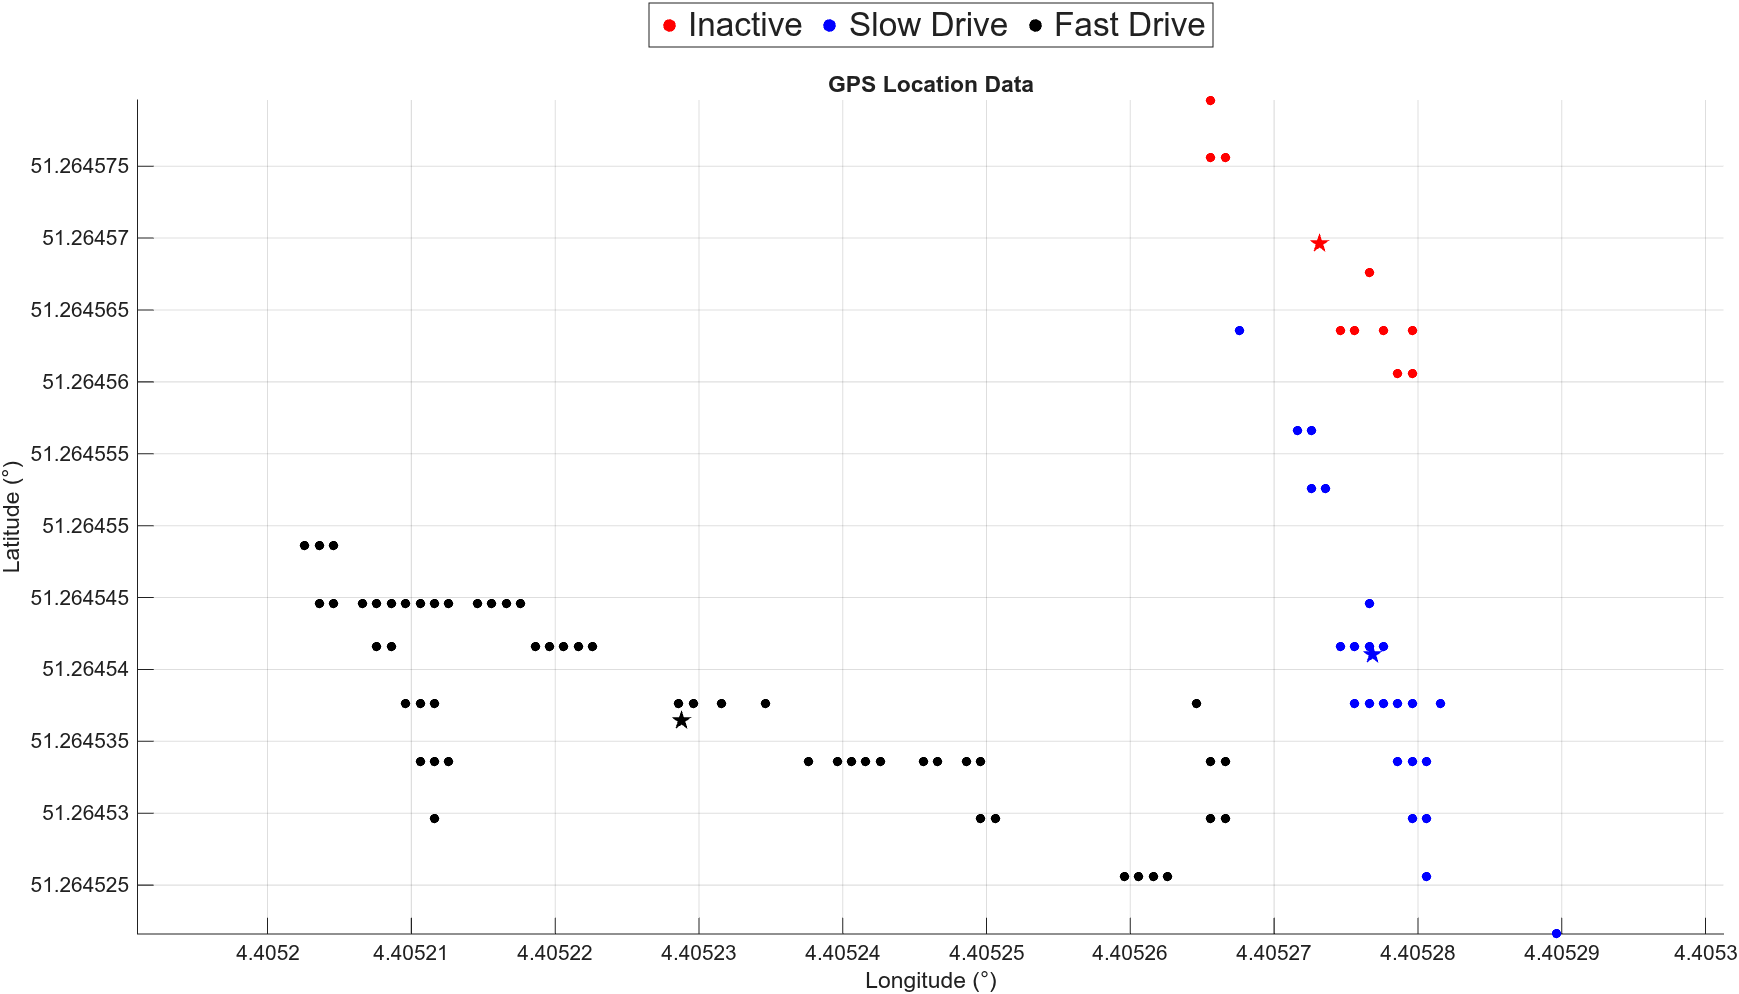
\includegraphics[width=\columnwidth]{images/stationary/exp_position.png}
	\caption{
		The positioning accuracy of the TruggySense V2, while stationary.
		The center point, of each data set, indicated by the pentagram.
	}
	\label{fig:exp_position}
\end{figure}

\begin{table}[!t]
	\centering
	\caption{Positioning deviation}
	\begin{threeparttable}
	\begin{tabular}{lccc}
		\toprule
			Distance to & Standstill (m) & Slow driving (m) & Fast driving (m) \\
		\midrule
			Centroid  & 1.23 & 2.59 & 2.74 \\
			Stationary & 0.00 & 3.19 & 4.81 \\
		\bottomrule
	\end{tabular}
	\begin{tablenotes}[leftmargin=*]
      	\footnotesize
		\item The data in the first row represents the distance from the centroid of each data set, compared to the furthest point in that data set.
      		  The data in the second row represents the distance of each centroid compared to the centroid of the stationary data set.
    \end{tablenotes}
	\end{threeparttable}
	\label{tab:position_distance}
\end{table}

\ParagraphSeperator
Fig.~\ref{fig:exp_wheels} illustrates the measured rotational speed of each wheel compared to the combined data set.
Across both the "Slow driving" and "Fast driving" experiments, the Front Right (FR) exhibited an above-average rotational speed, while that of the Front Left (FL) was below average.
Implying that, even while suspended, the system steers to the left.

\begin{figure}[!t]
	\centering
	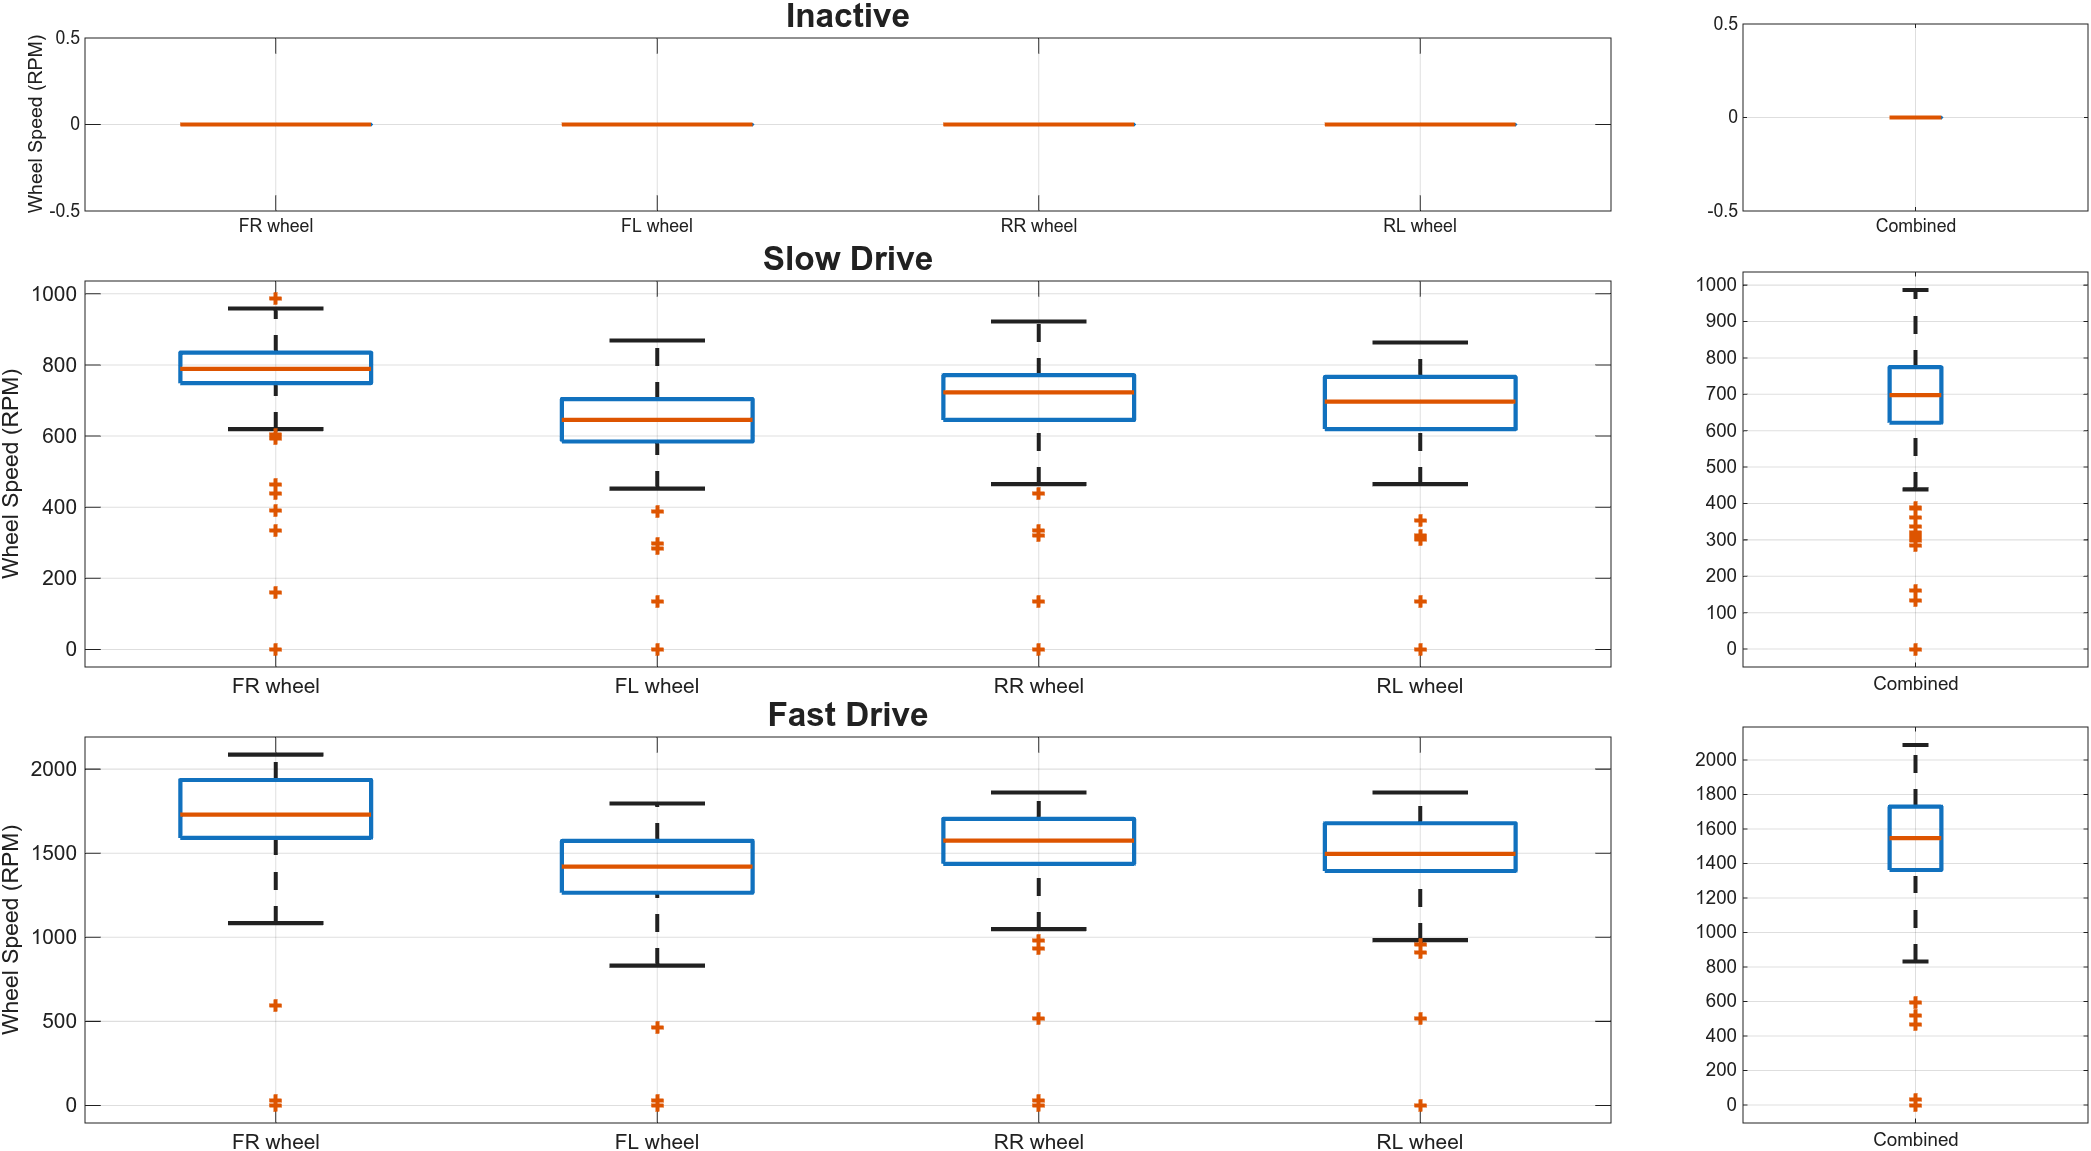
\includegraphics[width=\columnwidth]{images/stationary/exp_wheels.png}
	\caption{Accuracy of the wheel rotation of the TruggySense V2 while stationary.}
	\label{fig:exp_wheels}
\end{figure}

\ParagraphSeperator
Fig.~\ref{fig:exp_IMU} reveals the stability of the orientation angles, and that there are disturbances introduced by vibrations caused by the rotation of the wheels.
These disturbances increase and become more frequent with an increase in rotational speed.
Nevertheless, even for the "Fast drive" experiment, these deviations remain within approximately $\pm$1° across all orientation angles, implying that the placement of the IMU has no effect on its operational capabilities, and thus can be mounted to the PCB instead of the bottom the chassis.

\begin{figure}[!t]
	\centering
	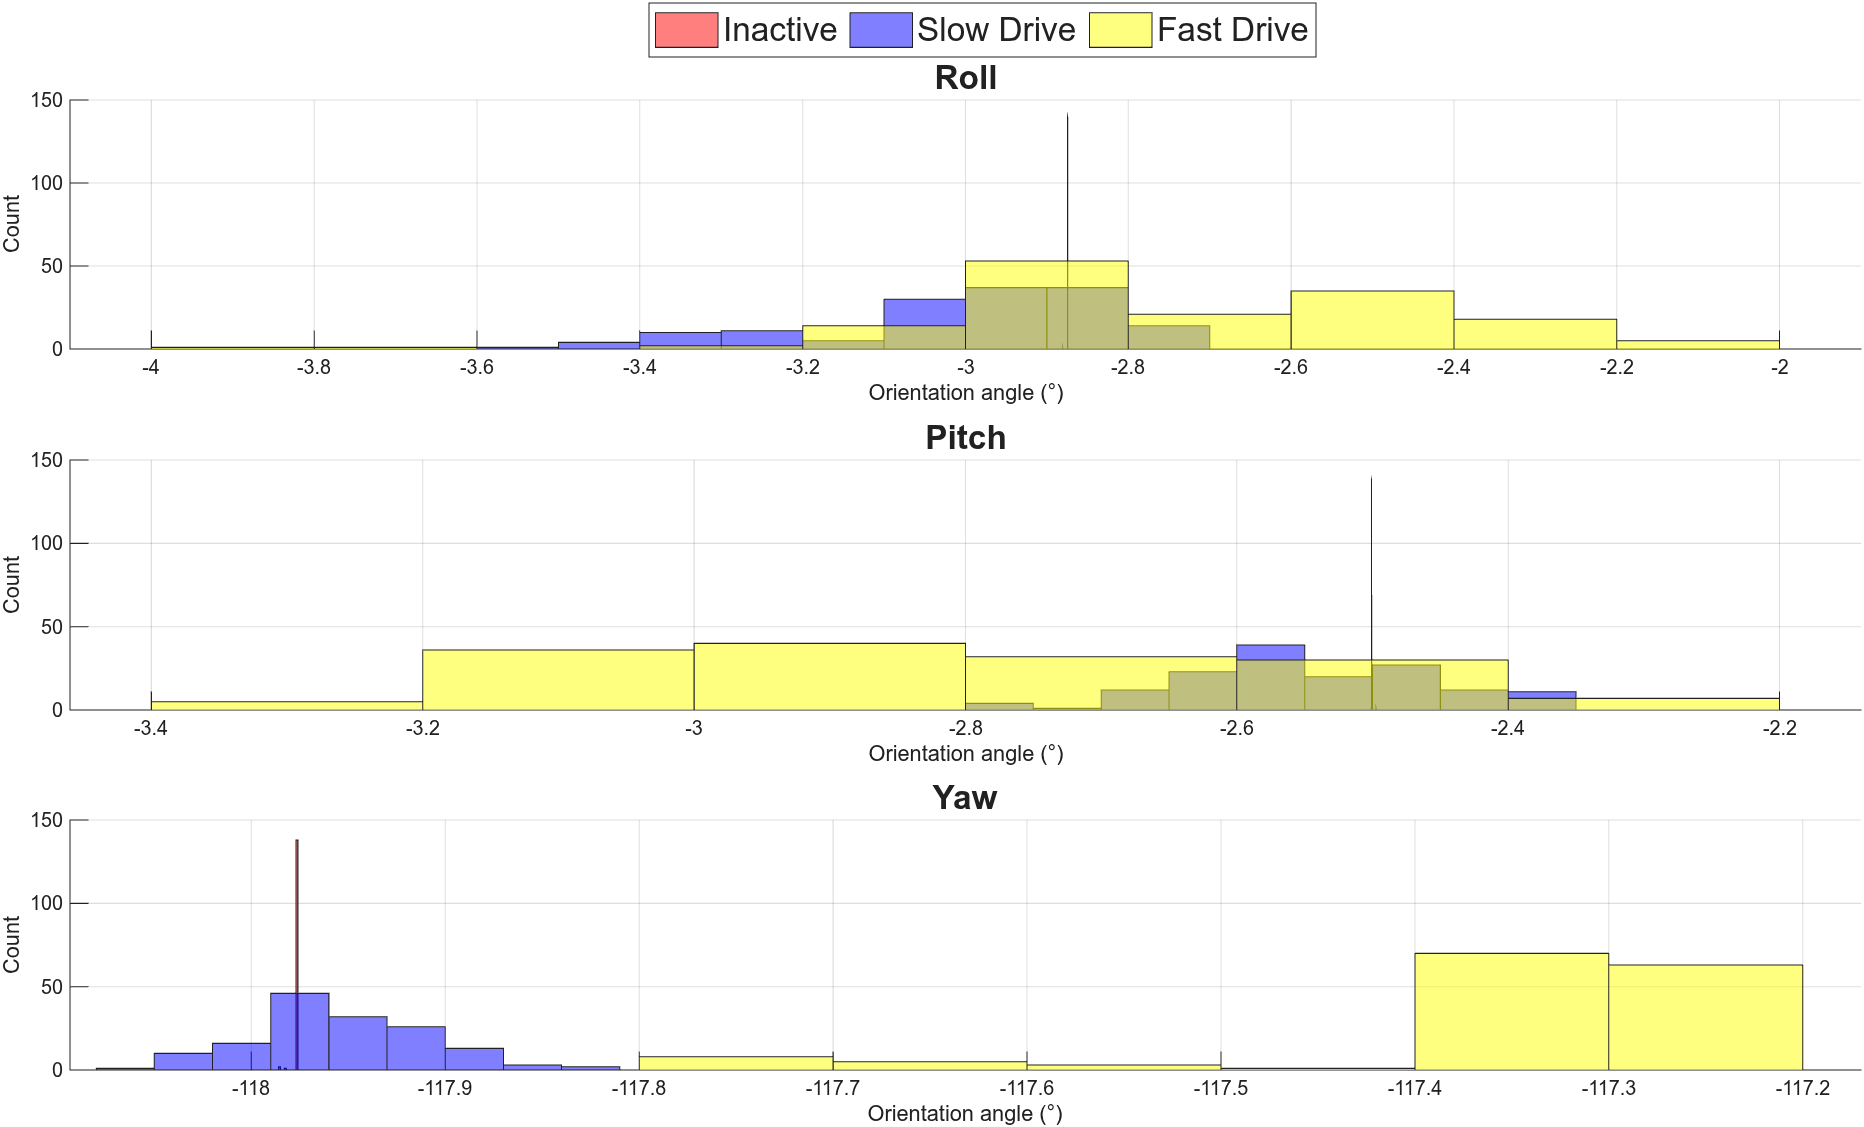
\includegraphics[width=\columnwidth]{images/stationary/exp_IMU.png}
	\caption{Accuracy of the orientation angles of the TruggySense V2 while stationary.}
	\label{fig:exp_IMU}
\end{figure}

\section{Discussion and Conclusion}
\ParagraphSeperator
This paper covers the modifications made to the TruggySense V1 and evaluates their impact on the DAQ.
It confirms that the system remains capable of ascertaining real-world behavior and key metrics, including driving speed, wheel slip, and orientation, while retaining its accuracy.
Furthermore, it introduces support for IWD and system expansion, while simplifying the hardware assembly.
On top of that, it reduces the overall complexity of the system, streamlining the integration of new modules in both hardware and firmware.

\ParagraphSeperator
However, several limitations still remain. 
It is still unclear whether the system supports reverse polarity protection, and while support for redundancy has been added, full redundancy has not been implemented. 
Additionally, another attempt at integrating ROS2 was made, but did not yield any discernible progress.
Beyond that, the losses introduced by the new temperature sensors do not justify the replacement of the old modules.

\ParagraphSeperator
This work continued on the solid foundation that was provided by the TruggySense V1, making it more approachable for the student who will continue to work on it.
Just like its predecessor, it did not focus on groundbreaking scientific discoveries but continued to build a foundation that has the potential to make an impact within the context of engineering education.
One enhancement that could be introduced is the addition of both RADAR and LiDAR technology.
This, in turn, would lay the groundwork for turning this RCV system into a fully autonomous vehicle, capable of comprehending and navigating any off-road environment.

\section{Acknowledgement}
Appreciation is extended to RC Racing Fun Bornem for allowing the TruggySense to be tested again on their RC off-road track.
This not only served as a consistent and controlled environment, but also as a great reference to the original research of Robbe Elsermans. 
The availability of this facility once again played a significant role in the improvement of the TruggySense.

\appendix

% \clearpage
\begin{minipage}{\linewidth}
	\vspace{6pt}
	\subsection{Render of the final PCB-design}
	\begin{center}
		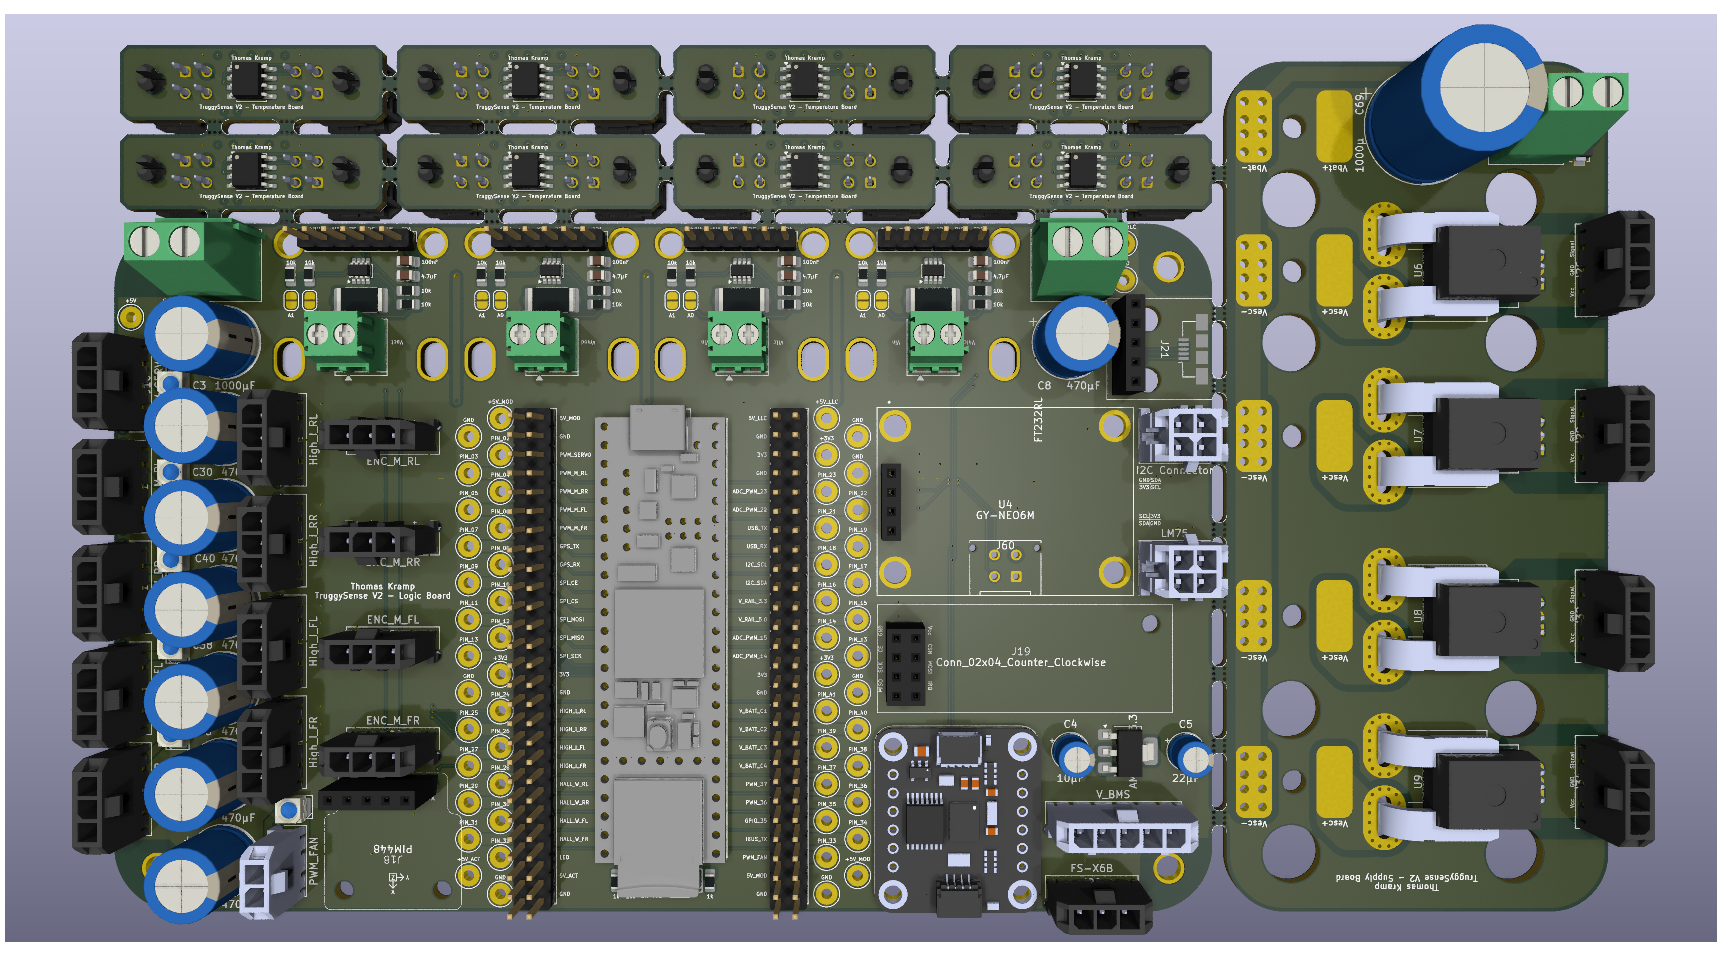
\includegraphics[width=\columnwidth]{images/appendix/board_logic_top.png}
		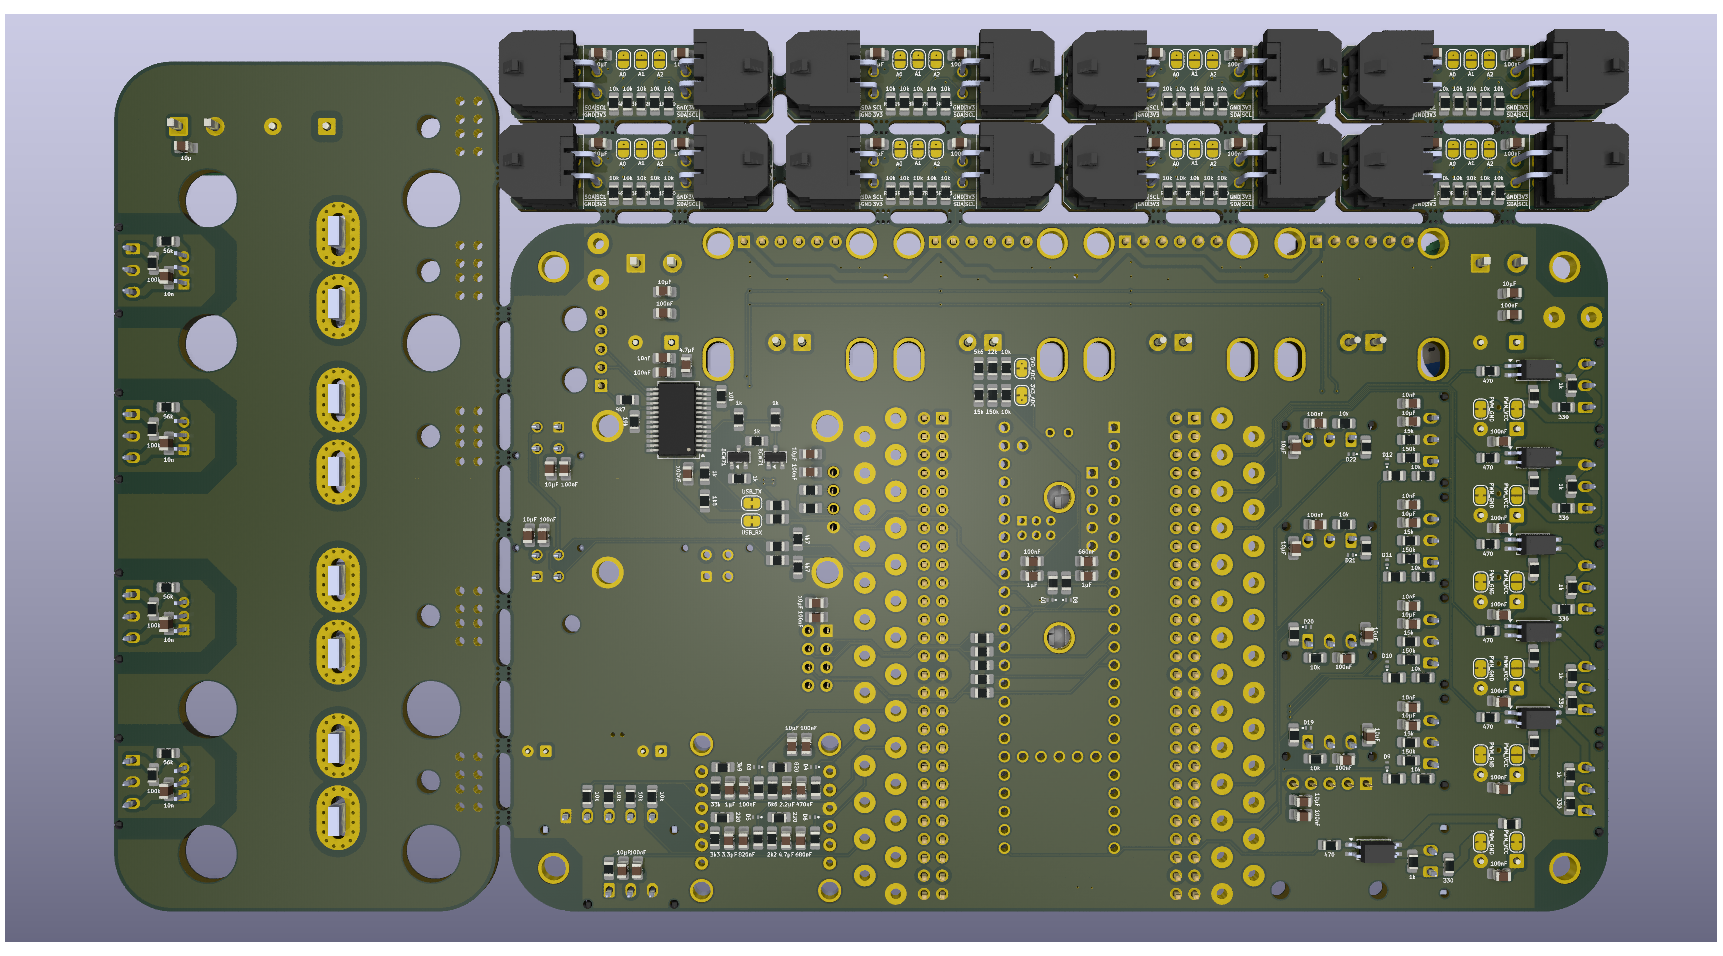
\includegraphics[width=\columnwidth]{images/appendix/board_logic_bottom.png}\vspace{-3pt}
		\captionof{figure}{3D render of the final PCB-design, displaying the top and bottom layer.}
		\label{fig:board_logic}
	\end{center}
	\vspace{6pt}
\end{minipage}

\begin{minipage}{\linewidth}
	\subsection{Proof of track width equation}
	\vspace{-18pt}
	\begin{align}
    \label{eq:proof_track_width}
		I 													  & = k \cdot \Delta T^{0.44} \cdot (W \cdot H)^{0.725} \\
		\frac{I}{k \cdot \Delta T^{0.44}} 					  & = (W \cdot H)^{0.725} \\
		(\frac{I}{k \cdot \Delta T^{0.44}})^{\frac{1}{0.725}} & = W \cdot H \\
		W 													  & = \frac{1}{H} \cdot (\frac{I}{k \cdot \Delta T^{0.44}})^{\frac{1}{0.725}}
	\end{align}
	\vspace{6pt}
\end{minipage}

\begin{minipage}{\linewidth}
	\subsection{Proof of via hole diameter equation}
	\vspace{-18pt}
	\begin{align}
    	\label{eq:proof_via_width}
		A & = A_{hole} - A_{hole - copper} \\
		  & = \pi \cdot (r_{hole}^{2} - (r_{hole} - t)^{2}) \\
		  & = \pi \cdot (r_{hole}^{2} - (r_{hole}^{2} - 2 \cdot r_{hole} \cdot t + t^{2})) \\
		  & = \pi \cdot (2 \cdot r_{hole} \cdot t - t^{2}) \\
		  & = \pi \cdot t \cdot (2 \cdot r_{hole} - t) \\
		  & = \pi \cdot t \cdot (d_{hole} - t)
	\end{align}
	\vspace{6pt}
\end{minipage}

\begin{minipage}{\linewidth}
	\subsection{Battery noise on supply}
	\begin{center}
		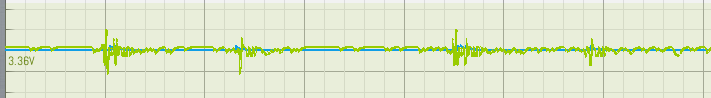
\includegraphics[width=\columnwidth]{images/appendix/supply_noise.png}\vspace{-3pt}
		\captionof{figure}{
			The 3.3V rail on the prototype of the logic board.
			The green signal represents the rail when the board is connected to the battery.
			The blue signal represents the rail when the board is disconnected from the battery.
		}
		\label{fig:supply_noise}
	\end{center}
	\vspace{6pt}
\end{minipage}

\begin{minipage}{\linewidth}
	\subsection{"Fast mode" straight line steering}
	\begin{center}
		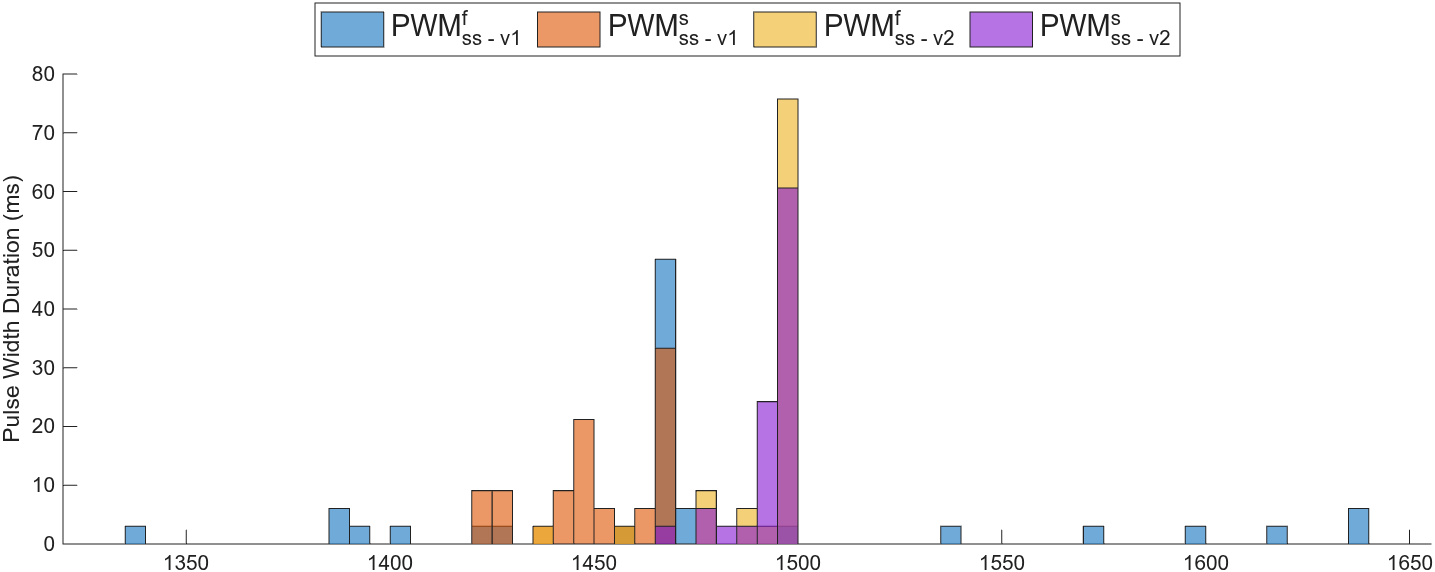
\includegraphics[width=\columnwidth]{images/experiments/exp2_fig3.png}\vspace{-3pt}
		\captionof{figure}{Distribution of fast and slow steer PWM value, between the TruggySense V1 and V2.}
		\label{fig:exp2_fig3}
	\end{center}
	\vspace{6pt}
\end{minipage}

\setlength{\parskip}{1em}
\setlength{\parindent}{0pt}
\bibliographystyle{IEEEtran}

\setlength{\parskip}{0em}
\setlength{\parindent}{0pt}
\bibliography{bibliography}

\end{document}
